%% DoggoGO – Diplomarbeit
%% Kandidat: Daniel Hoheneder
%% Betreuer: [Betreuer eintragen]
%% HTL Leonding, 2024/25

\documentclass[12pt, a4paper, oneside]{report}

%% -------------------------------------------------------
%% Pakete
%% -------------------------------------------------------
\usepackage[utf8]{inputenc}
\usepackage[T1]{fontenc}
\usepackage[ngerman]{babel}
\usepackage{lmodern}
\usepackage{geometry}
\geometry{top=3cm, bottom=3cm, left=3.5cm, right=2.5cm}

\usepackage{graphicx}
\usepackage{float}
\usepackage{caption}
\usepackage{subcaption}
\usepackage{booktabs}
\usepackage{tabularx}
\usepackage{longtable}
\usepackage{array}
\usepackage{multirow}

%% Tabellen: raggedright X-Spalte (verhindert Overfull hbox)
\newcolumntype{Y}{>{\raggedright\arraybackslash}X}
\newcolumntype{Z}{>{\centering\arraybackslash}X}
\renewcommand{\arraystretch}{1.3}

%% TikZ für Diagramme
\usepackage{tikz}
\usetikzlibrary{shapes.geometric, shapes.multipart, arrows.meta, positioning, fit, calc, er}

\usepackage{listings}
\usepackage{xcolor}

\usepackage{amsmath}
\usepackage{amssymb}

\usepackage[hyphens]{url}
\usepackage[
  pdftitle={DoggoGO – Diplomarbeit Daniel Hoheneder},
  pdfauthor={Daniel Hoheneder},
  colorlinks=true,
  linkcolor=black,
  citecolor=black,
  urlcolor=blue
]{hyperref}

\usepackage{csquotes}
\usepackage[backend=biber, style=ieee, sorting=none]{biblatex}
\addbibresource{bibliography.bib}

\usepackage{setspace}
\onehalfspacing

\usepackage{fancyhdr}
\setlength{\headheight}{14.5pt}
\pagestyle{fancy}
\fancyhf{}
\fancyhead[R]{\thepage}
\fancyhead[L]{\nouppercase{\rightmark}}
\renewcommand{\headrulewidth}{0.4pt}

\usepackage{parskip}
\setlength{\parskip}{6pt}

%% -------------------------------------------------------
%% Code-Listing Stil
%% -------------------------------------------------------
\definecolor{codegreen}{rgb}{0,0.6,0}
\definecolor{codegray}{rgb}{0.5,0.5,0.5}
\definecolor{codepurple}{rgb}{0.58,0,0.82}
\definecolor{backcolour}{rgb}{0.97,0.97,0.97}

\lstdefinestyle{mystyle}{
  backgroundcolor=\color{backcolour},
  commentstyle=\color{codegreen},
  keywordstyle=\color{blue}\bfseries,
  numberstyle=\tiny\color{codegray},
  stringstyle=\color{codepurple},
  basicstyle=\ttfamily\footnotesize,
  breakatwhitespace=false,
  breaklines=true,
  captionpos=b,
  keepspaces=true,
  numbers=left,
  numbersep=5pt,
  showspaces=false,
  showstringspaces=false,
  showtabs=false,
  tabsize=2,
  frame=single,
  rulecolor=\color{codegray}
}
\lstset{style=mystyle,
  extendedchars=true,
  literate={—}{{-}}1 {–}{{-}}1 {→}{{->}}2 {…}{{...}}3
           {ä}{{\"a}}1 {ö}{{\"o}}1 {ü}{{\"u}}1
           {Ä}{{\"A}}1 {Ö}{{\"O}}1 {Ü}{{\"U}}1 {ß}{{\ss}}1
}

\lstdefinelanguage{csharp}{
  keywords={abstract, as, base, bool, break, byte, case, catch, char, checked,
    class, const, continue, decimal, default, delegate, do, double, else,
    enum, event, explicit, extern, false, finally, fixed, float, for, foreach,
    goto, if, implicit, in, int, interface, internal, is, lock, long, namespace,
    new, null, object, operator, out, override, params, private, protected,
    public, readonly, ref, return, sbyte, sealed, short, sizeof, stackalloc,
    static, string, struct, switch, this, throw, true, try, typeof, uint,
    ulong, unchecked, unsafe, ushort, using, virtual, void, volatile, while,
    async, await, var, get, set, value},
  sensitive=true,
  morecomment=[l]{//},
  morecomment=[s]{/*}{*/},
  morestring=[b]",
  morestring=[b]'
}

\lstdefinelanguage{swift}{
  keywords={class, struct, enum, protocol, extension, func, var, let, if, else,
    for, while, return, import, self, super, init, deinit, get, set, willSet,
    didSet, throws, throw, try, catch, guard, where, in, is, as, nil, true,
    false, typealias, associatedtype, some, any, async, await, actor, override,
    final, open, public, internal, private, fileprivate, static, lazy, weak,
    unowned, mutating, nonmutating, convenience, required, optional, indirect,
    @State, @Binding, @ObservedObject, @StateObject, @EnvironmentObject,
    @Published, @ViewBuilder, @MainActor, View, Text, VStack, HStack, ZStack,
    Button, NavigationView, NavigationLink, List, Map, MapKit},
  sensitive=true,
  morecomment=[l]{//},
  morecomment=[s]{/*}{*/},
  morestring=[b]",
  morestring=[b]'
}

%% -------------------------------------------------------
%% Titelseite
%% -------------------------------------------------------
\begin{document}

\begin{titlepage}
  \centering
  
\includegraphics[width=5cm]{images/htl_leo_logo.png}\\[1.5cm]
  {\large \textbf{HTL Leonding}\\
  Höhere Technische Bundeslehr- und Versuchsanstalt Leonding}\\[0.5cm]
  {\large Abteilung Informatik}\\[2cm]

  {\LARGE \textbf{Diplomarbeit}}\\[0.5cm]
  {\Huge \textbf{DoggoGO}}\\[0.3cm]
  {\large Eine standortbasierte Web- und iOS-App für Hundehalter}\\[2cm]

  \begin{tabular}{ll}
    \textbf{Kandidat:}   & Daniel Hoheneder \\[0.3cm]
    \textbf{Betreuer:}   & Stöttinger Robert \\[0.3cm]
    \textbf{Schuljahr:}  & 2025/26 \\[0.3cm]
    \textbf{Abgabedatum:} & 26.03.2026 \\
  \end{tabular}

  \vfill
  {\small Eingereicht an der HTL Leonding zur Erlangung des\\
  akademischen Grades \textit{Ingenieur/in}}
\end{titlepage}

%% -------------------------------------------------------
%% Eidesstattliche Erklärung
%% -------------------------------------------------------
\chapter*{Eidesstattliche Erklärung}
\addcontentsline{toc}{chapter}{Eidesstattliche Erklärung}

Ich erkläre an Eides statt, dass ich die vorliegende Diplomarbeit selbstständig und ohne fremde
Hilfe verfasst, andere als die angegebenen Quellen und Hilfsmittel nicht benutzt und die den
benutzten Quellen wörtlich oder inhaltlich entnommenen Stellen als solche kenntlich gemacht habe.

Leonding, am 26.03.2026 

\vspace{1cm}
\underline{\hspace{6cm}}\\
Daniel Hoheneder

\clearpage

%% -------------------------------------------------------
%% Abstract
%% -------------------------------------------------------
%% -------------------------------------------------------
%% Kapitel 0: Abstract (DE + EN)
%% -------------------------------------------------------
\chapter*{Kurzfassung}
\addcontentsline{toc}{chapter}{Kurzfassung}

Die vorliegende Diplomarbeit beschreibt die Entwicklung von \textbf{DoggoGO}, einer standortbasierten
Plattform für Hundehalter\-innen und Hundehalter. Das Ziel der Anwendung ist es, relevante
Informationen – wie die Positionen von Freilaufwiesen, Sackerlspendern und Hundekot-Müllbehältern
sowie rassenspezifische gesetzliche Vorschriften (Leinen- und Maulkorbpflicht) – in Echtzeit und
standortgebunden bereitzustellen.

Dieser Teil der Arbeit behandelt die technische Umsetzung des \textbf{Backends} auf Basis von
\textbf{ASP.NET~Core~8} sowie die Entwicklung der \textbf{iOS-Applikation} mit \textbf{Swift} und
\textbf{SwiftUI}. Das Backend stellt eine RESTful~API bereit, die von der Angular-Webapplikation
(von Manuel Rankl) und der iOS-App konsumiert wird. Als Persistenzschicht kommt \textbf{PostgreSQL}
in Kombination mit \textbf{Entity~Framework~Core~9} zum Einsatz. Die gesamte Serverinfrastruktur
wird mittels \textbf{Docker} containerisiert und betrieben.

Die iOS-App ermöglicht die Kartenansicht mit standortbasierten Markierungen über \textbf{MapKit},
die Verwaltung von Hundeprofilen sowie die Anzeige rassenspezifischer Rechtsvorschriften. Die
Authentifizierung erfolgt über \textbf{JSON~Web~Tokens~(JWT)}.

\vspace{1.5em}
\noindent\textit{Schlagwörter: ASP.NET Core, Entity Framework Core, PostgreSQL, Docker, iOS, SwiftUI,
MapKit, JWT, REST~API, Geofencing}

\clearpage

%% -------------------------------------------------------
%% Abstract (English)
%% -------------------------------------------------------
\chapter*{Abstract}
\addcontentsline{toc}{chapter}{Abstract}

This diploma thesis describes the development of \textbf{DoggoGO}, a location-based platform for
dog owners. The application aims to provide relevant information in real time – such as the
locations of off-leash areas, poop-bag dispensers, and dog waste bins, as well as
breed-specific legal regulations (leash and muzzle requirements) – based on the user's current
location.

This part of the thesis covers the technical implementation of the \textbf{backend} using
\textbf{ASP.NET~Core~8} and the development of the \textbf{iOS application} using \textbf{Swift}
and \textbf{SwiftUI}. The backend exposes a RESTful~API consumed by both the Angular web
application (developed by Manuel Rankl) and the iOS app. \textbf{PostgreSQL} together with
\textbf{Entity~Framework~Core~9} serves as the persistence layer. The entire server
infrastructure is containerised and operated using \textbf{Docker}.

The iOS app provides a map view with location-based markers via \textbf{MapKit}, dog profile
management, and the display of breed-specific legal requirements. Authentication is handled
via \textbf{JSON~Web~Tokens~(JWT)}.

\vspace{1.5em}
\noindent\textit{Keywords: ASP.NET Core, Entity Framework Core, PostgreSQL, Docker, iOS, SwiftUI,
MapKit, JWT, REST~API, Geofencing}

\clearpage


%% -------------------------------------------------------
%% Inhaltsverzeichnis
%% -------------------------------------------------------
\tableofcontents
\clearpage

\listoffigures
\addcontentsline{toc}{chapter}{Abbildungsverzeichnis}
\clearpage

\listoftables
\addcontentsline{toc}{chapter}{Tabellenverzeichnis}
\clearpage

\lstlistoflistings
\addcontentsline{toc}{chapter}{Quellcodeverzeichnis}
\clearpage

%% -------------------------------------------------------
%% Kapitel – Daniels Teil (Backend & iOS)
%% -------------------------------------------------------
%% -------------------------------------------------------
%% Kapitel 1: Einleitung
%% -------------------------------------------------------
\chapter{Einleitung}
\label{chap:einleitung}

\section{Ausgangssituation und Problemstellung}
\label{sec:ausgangssituation}

Wer mit einem Hund in einer österreichischen Stadt oder Gemeinde unterwegs ist, sieht sich
täglich mit einer Vielzahl praktischer Fragen konfrontiert: Wo befindet sich die nächste
Freilaufwiese, auf der der Hund ohne Leine toben darf? Gibt es in der Nähe einen
Hundekot-Müllbehälter oder einen Sackerlspender? Und – besonders relevant für Halter\-innen
und Halter bestimmter Rassen – gilt an diesem Ort eine Leinen- oder Maulkorbpflicht für
ihren Hund?

Diese Informationen sind zwar grundsätzlich verfügbar, aber über viele verschiedene Quellen
verstreut: kommunale Webseiten, amtliche Kundmachungen, geografische Open-Data-Portale oder
mündliche Weitergabe unter Hundehalter\-innen und Hundehaltern. Eine zentrale, standortbewusste
und rassenspezifische Anlaufstelle fehlt im deutschsprachigen App-Markt weitgehend.

\subsection{Defizite bestehender Lösungen}
\label{subsec:defizite}

Eine Analyse verfügbarer Anwendungen zeigt, dass keine der bekannten Lösungen alle
relevanten Anforderungen in einer einzigen App vereint:

\begin{table}[H]
  \centering
  \caption{Vergleich bestehender Lösungen}
  \label{tab:konkurrenzanalyse}
  \small
  \begin{tabularx}{\textwidth}{|p{2.8cm}|Y|Y|Y|Y|}
    \hline
    \textbf{App / Dienst} & \textbf{Karte mit POIs} & \textbf{Rechtsvorgaben} &
    \textbf{Rassenfilter} & \textbf{iOS-App} \\
    \hline
    BringGassi       & Ja (wenige) & Nein & Nein & Ja \\
    \hline
    Google Maps      & Nein        & Nein & Nein & Ja \\
    \hline
    Open\-Street\-Map & Begrenzt   & Nein & Nein & Indirekt \\
    \hline
    Wien.gv.at       & Ja (Wien)   & Begrenzt & Nein & Nein \\
    \hline
    \textbf{DoggoGO} & \textbf{Ja} & \textbf{Ja} & \textbf{Ja} & \textbf{Ja} \\
    \hline
  \end{tabularx}
\end{table}

\textbf{BringGassi} bietet zwar eine kartenzentrierte Ansicht für Hundeausflüge, deckt
jedoch keine rechtlichen Vorgaben ab und ist regional stark begrenzt. \textbf{Google Maps}
erlaubt grundsätzlich die Suche nach Hundeauslaufzonen, verfügt aber über keinerlei
rassenspezifische Rechtsinformationen und ist nicht auf Hundehaltung spezialisiert. Kommunale
Portale wie das der Stadt Wien bieten Standortdaten für ihren Zuständigkeitsbereich, sind
aber weder mobil optimiert noch rassenspezifisch und nicht überregional einsetzbar.

Das Kerndefizit aller betrachteten Lösungen liegt in der fehlenden Verknüpfung von drei
Aspekten, die Hundehalter\-innen und Hundehalter täglich benötigen:
\begin{enumerate}
  \item standortbezogene Karte mit relevanten Points of Interest (POIs),
  \item rassenspezifische gesetzliche Informationen (Leinen-/Maulkorbpflicht),
  \item plattformübergreifende Verfügbarkeit (Web \emph{und} iOS).
\end{enumerate}

\section{Zielsetzung dieser Arbeit}
\label{sec:zielsetzung}

Diese Diplomarbeit behandelt die Realisierung von zwei zentralen Komponenten des
DoggoGO-Projekts: dem \textbf{Backend} und der \textbf{iOS-Applikation}.

Das \textbf{Backend} hat folgende Aufgaben:
\begin{itemize}
  \item Bereitstellung einer RESTful~API für die Angular-Webanwendung und die iOS-App,
  \item Verwaltung von Hundehalter\-innen und Hundehaltern sowie ihrer Hundeprofile,
  \item Persistenz der Hunderassen inklusive ihrer rassenspezifischen Rechtsvorschriften,
  \item sicherer Betrieb in einer Docker-Container-Umgebung.
\end{itemize}

Die \textbf{iOS-App} soll:
\begin{itemize}
  \item eine interaktive Karte mit standortbasierten Markierungen (Freilaufwiesen,
        Sackerlspender, Hundekot-Müllbehälter) anzeigen,
  \item das Hundeprofil der Nutzerin / des Nutzers verwalten,
  \item rassenspezifische Leinen- und Maulkorbvorschriften für den aktuellen Standort anzeigen,
  \item eine sichere Anmeldung per JWT-Authentifizierung bieten.
\end{itemize}

\section{Abgrenzung}
\label{sec:abgrenzung}

Die Angular-Webanwendung (inklusive UI/UX-Konzept, Routenplanung, Wetterintegration und
Progressive-Web-App-Funktionalität) wurde von Manuel Rankl entwickelt und ist nicht
Gegenstand dieser Arbeit. Gleiches gilt für die Entwicklung eines Android-Clients. Das in
dieser Arbeit beschriebene Backend bildet die gemeinsame Datenbasis für beide Frontends.

\section{Aufbau der Arbeit}
\label{sec:aufbau}

Die vorliegende Arbeit ist wie folgt gegliedert:

\begin{description}
  \item[Kapitel~\ref{chap:anforderungen} – Anforderungsanalyse:]
    Beschreibung der Stakeholder, funktionaler und nicht-funktionaler Anforderungen sowie
    der Use-Case-Szenarien aus Sicht des Backends und der iOS-App.
  \item[Kapitel~\ref{chap:architektur} – Systemarchitektur:]
    Gesamtarchitektur der Plattform, Datenbankdesign, REST-API-Überblick und
    Kommunikationsfluss zwischen den Systemkomponenten.
  \item[Kapitel~\ref{chap:technologie} – Technologieauswahl:]
    Begründete Auswahl der eingesetzten Technologien (ASP.NET~Core~8, Entity~Framework~Core~9,
    PostgreSQL, iOS/SwiftUI) mit Bewertung von Alternativen.
  \item[Kapitel~\ref{chap:backend} – Backend-Implementierung:]
    Detaillierte Beschreibung der API-Endpunkte, Datenbankmodelle, Migrations,
    Authentifizierung, Breed-Seeding und Docker-Deployment.
  \item[Kapitel~\ref{chap:ios} – iOS-Applikation:]
    Architektur und Implementierung der iOS-App: MapKit-Integration, Standortdienste,
    Authentifizierungsflow und Hundeprofilverwaltung.
  \item[Kapitel~\ref{chap:testing} – Testing und Deployment:]
    Teststrategie, durchgeführte Tests und Erkenntnisse aus dem Deployment.
  \item[Kapitel~\ref{chap:zusammenfassung} – Zusammenfassung:]
    Reflexion der erreichten Ziele, suboptimaler Entscheidungen, Einschränkungen und
    Erweiterungsmöglichkeiten.
\end{description}

%% -------------------------------------------------------
%% Kapitel 2: Anforderungsanalyse
%% -------------------------------------------------------
\chapter{Anforderungsanalyse}
\label{chap:anforderungen}

Dieses Kapitel beschreibt die Anforderungen an das Backend und die iOS-App von DoggoGO.
Die Erhebung erfolgte auf Basis des Projektvorschlags, des Product Backlogs sowie eigener
Überlegungen zu Sicherheit, Performance und Wartbarkeit.

\section{Stakeholder und Zielgruppe}
\label{sec:stakeholder}

Die wichtigsten Stakeholder des Projekts sind:

\begin{description}
  \item[Hundehalter\-innen und Hundehalter (Endnutzer\-innen/-nutzer)]
    Personen, die mit einem oder mehreren Hunden in urbanen oder ländlichen Gebieten
    unterwegs sind und standortbezogene Informationen benötigen. Sie interagieren mit der
    Plattform über die Webapplikation oder die iOS-App.
  \item[Entwicklerinnen und Entwickler]
    Das Projektteam (Manuel Rankl für das Angular-Frontend, Daniel Hoheneder für Backend
    und iOS). Anforderungen an Wartbarkeit, klare API-Contracts und gute Dokumentation
    sind daher ebenso relevant.
  \item[HTL Leonding (Auftraggeber)]
    Die Schule als Auftraggeber und Bewerter der Diplomarbeit erwartet eine technisch
    fundierte, vollständig dokumentierte Lösung, die die im Projektvorschlag definierten
    Ziele erfüllt.
\end{description}

\section{Funktionale Anforderungen}
\label{sec:funktionale-anforderungen}

\subsection{Backend-API}
\label{subsec:fa-backend}

\begin{table}[H]
  \centering
  \caption{Funktionale Anforderungen – Backend}
  \label{tab:fa-backend}
  \begin{tabularx}{\textwidth}{|l|Y|}
    \hline
    \textbf{ID} & \textbf{Anforderung} \\
    \hline
    FA-B01 & Das System muss eine RESTful~API bereitstellen, die von der Angular-Webanwendung
             und der iOS-App konsumiert werden kann. \\
    \hline
    FA-B02 & Nutzer\-innen und Nutzer müssen sich mit E-Mail-Adresse und Passwort registrieren
             und anmelden können. \\
    \hline
    FA-B03 & Nach erfolgreicher Anmeldung muss ein JWT ausgestellt werden, das alle
             nachfolgenden Anfragen autorisiert. \\
    \hline
    FA-B04 & Angemeldete Nutzer\-innen und Nutzer müssen Hundeprofile (Name, Alter, Rasse)
             anlegen, lesen, aktualisieren und löschen können (CRUD). \\
    \hline
    FA-B05 & Das System muss eine Liste aller verfügbaren Hunderassen mit deren Beschreibung
             und rassenspezifischen Rechtsvorschriften liefern. \\
    \hline
    FA-B06 & Rasseninformationen müssen beim ersten Start aus einer JSON-Datei automatisch
             in die Datenbank eingelesen werden (Seeding). \\
    \hline
    FA-B07 & Das Backend muss in einem Docker-Container lauffähig sein und mit einer
             ebenfalls containerisierten PostgreSQL-Instanz kommunizieren. \\
    \hline
    FA-B08 & Die API-Endpunkte müssen über Swagger~(OpenAPI) dokumentiert und testbar sein. \\
    \hline
  \end{tabularx}
\end{table}

\subsection{iOS-Applikation}
\label{subsec:fa-ios}

\begin{table}[H]
  \centering
  \caption{Funktionale Anforderungen – iOS-App}
  \label{tab:fa-ios}
  \begin{tabularx}{\textwidth}{|l|Y|}
    \hline
    \textbf{ID} & \textbf{Anforderung} \\
    \hline
    FA-I01 & Die App muss eine interaktive Karte anzeigen (DOG1). \\
    \hline
    FA-I02 & Der eigene Standort muss auf der Karte dargestellt werden (DOG2). \\
    \hline
    FA-I03 & Nutzer\-innen und Nutzer müssen sich in der App registrieren und anmelden
             können. \\
    \hline
    FA-I04 & Angemeldete Nutzer\-innen und Nutzer müssen Hundeprofile verwalten können. \\
    \hline
    FA-I05 & Die App muss die Maulkorb- und Leinenpflicht für die gespeicherte Rasse und
             den aktuellen Standort anzeigen (DOG6). \\
    \hline
    FA-I06 & Nutzer\-innen und Nutzer müssen aus einer Liste von Hunderassen auswählen
             können (DOG8). \\
    \hline
    FA-I07 & Die App muss mit dem Backend über die bereitgestellte REST-API kommunizieren. \\
    \hline
    FA-I08 & Sitzungen müssen durch Speicherung des JWT persistent über App-Neustarts
             hinaus erhalten bleiben. \\
    \hline
  \end{tabularx}
\end{table}

\section{Nicht-funktionale Anforderungen}
\label{sec:nfas}

\begin{table}[H]
  \centering
  \caption{Nicht-funktionale Anforderungen}
  \label{tab:nfas}
  \begin{tabularx}{\textwidth}{|l|l|Y|}
    \hline
    \textbf{ID} & \textbf{Kategorie} & \textbf{Anforderung} \\
    \hline
    NF-01 & Sicherheit   & Passwörter dürfen nicht im Klartext gespeichert werden.
                           Es wird HMAC-SHA512 mit individuellem Salt eingesetzt. \\
    \hline
    NF-02 & Sicherheit   & JWTs müssen mit einem serverseitigen Secret signiert sein und
                           eine konfigurierbare Ablaufzeit besitzen. \\
    \hline
    NF-03 & Datenschutz  & Die App darf Standortdaten nur mit expliziter Zustimmung der
                           Nutzerin / des Nutzers erfassen (DSGVO, DOG12). \\
    \hline
    NF-04 & Performance  & API-Antworten müssen unter normalen Bedingungen in unter
                           500\,ms eintreffen. \\
    \hline
    NF-05 & Wartbarkeit  & Der Quellcode muss in einem öffentlichen Git-Repository
                           versioniert sein; Commits müssen nachvollziehbar beschrieben
                           werden. \\
    \hline
    NF-06 & Portierbarkeit & Das Backend muss plattformunabhängig über Docker deploybar
                           sein. \\
    \hline
    NF-07 & Kompatibilität & Die iOS-App muss auf Geräten ab iOS~16 lauffähig sein. \\
    \hline
    NF-08 & Erweiterbarkeit & Die Datenbankmodelle und API-Endpunkte müssen so gestaltet
                           sein, dass neue Entitäten (z.\,B.\ Standorte, Events) ohne
                           Breaking~Changes ergänzt werden können. \\
    \hline
  \end{tabularx}
\end{table}

\section{Use-Case-Szenarien}
\label{sec:use-cases}

Abbildung~\ref{fig:use-case} zeigt die wesentlichen Use Cases aus Sicht der Backend- und
iOS-Komponenten.

\begin{figure}[H]
  \centering
  \begin{tikzpicture}[
      actor/.style={draw, rectangle, rounded corners=6pt,
                    minimum width=2.8cm, minimum height=0.7cm,
                    align=center, font=\small},
      uc/.style={draw, ellipse, minimum width=3.2cm, minimum height=0.8cm,
                 align=center, font=\small},
      sys/.style={draw, dashed, rectangle, rounded corners=2pt,
                  inner sep=8pt, font=\small\itshape},
      arr/.style={-{Stealth[length=5pt]}, thin}
    ]
    % Akteur links
    \node[actor] (user) at (0,0) {Nutzer\-in / Nutzer};

    % System-Rahmen
    \node[sys, fit={(3,-2.5)(9,2.5)}] (sys) {};
    \node[font=\footnotesize\itshape] at (6, 2.2) {DoggoGO (iOS-App + Backend)};

    % Use Cases
    \node[uc] (uc1) at (6, 1.6) {Registrieren};
    \node[uc] (uc2) at (6, 0.7) {Anmelden};
    \node[uc] (uc3) at (6,-0.2) {Hund anlegen};
    \node[uc] (uc4) at (6,-1.1) {Rasse auswählen};
    \node[uc] (uc5) at (6,-2.0) {Vorschriften abrufen};

    % Verbindungen
    \foreach \uc in {uc1,uc2,uc3,uc4,uc5}
      \draw[arr] (user) -- (\uc);
  \end{tikzpicture}
  \caption{Use-Case-Diagramm – Backend und iOS-App}
  \label{fig:use-case}
\end{figure}

Die wichtigsten Szenarien sind:

\paragraph{UC-01: Registrierung}
Eine neue Nutzerin / ein neuer Nutzer öffnet die iOS-App, gibt Name, E-Mail und Passwort ein
und sendet die Anfrage an \texttt{POST /api/owners/register}. Das Backend validiert die
Eingaben, hasht das Passwort und legt einen neuen \texttt{Owner}-Datensatz an. Die App erhält
eine Erfolgsantwort und leitet zur Anmeldeseite weiter.

\paragraph{UC-02: Anmeldung und Kartenzugriff}
Die Nutzerin / der Nutzer meldet sich mit E-Mail und Passwort an (\texttt{POST /api/owners/login}).
Das Backend prüft den Passwort-Hash und stellt bei Übereinstimmung ein JWT aus. Die iOS-App
speichert das Token im \texttt{Keychain} und nutzt es für alle weiteren Anfragen. Anschließend
wird die Kartenansicht mit dem aktuellen Standort geladen.

\paragraph{UC-03: Hundeprofil anlegen}
Nach der Anmeldung wählt die Nutzerin / der Nutzer aus der Rassenliste eine Hunderasse aus
(\texttt{GET /api/breeds}) und erstellt ein Hundeprofil (\texttt{POST /api/dogs}). Der
Datensatz wird in der Datenbank gespeichert und der iOS-App bestätigt.

\paragraph{UC-04: Rechtliche Einschränkungen abrufen}
Die iOS-App ruft für die gespeicherte Hunderasse die \texttt{LegalRestrictions} ab und zeigt
Leinen- und Maulkorbvorschriften für den aktuellen Standort an.

%% -------------------------------------------------------
%% Kapitel 3: Systemarchitektur
%% -------------------------------------------------------
\chapter{Systemarchitektur}
\label{chap:architektur}

\section{Gesamtarchitektur}
\label{sec:gesamtarchitektur}

DoggoGO folgt einer klassischen \textbf{Client-Server-Architektur} mit drei Schichten:
einem Web-Frontend (Angular), einer nativen iOS-App und einem gemeinsamen Backend-Server,
der über eine REST-API kommuniziert. Die Datenhaltung erfolgt in einer PostgreSQL-Datenbank.
Abbildung~\ref{fig:gesamtarchitektur} illustriert die Systemkomponenten und deren Beziehungen.

\begin{figure}[H]
  \centering
  \begin{tikzpicture}[
      comp/.style={draw, rectangle, rounded corners=4pt,
                   minimum width=3.2cm, minimum height=0.9cm,
                   align=center, fill=gray!10, font=\small, text width=3cm},
      arr/.style={-{Stealth[length=5pt]}, thick},
      label/.style={font=\footnotesize\itshape, pos=0.65, above}
    ]
    \node[comp] (ios)     at (0, 1.2)  {iOS-App\\(Swift/SwiftUI)};
    \node[comp] (angular) at (0,-1.2)  {Angular\\Web-App};
    \node[comp] (api)     at (5, 0)    {Backend-API\\(ASP.NET Core 8)};
    \node[comp] (db)      at (10, 0)   {PostgreSQL\\Datenbank};

    \draw[arr] (ios)     -- node[label, yshift=5pt]{HTTP/JSON} (api);
    \draw[arr] (angular) -- node[label, below, yshift=-5pt]{HTTP/JSON} (api);
    \draw[arr] (api)     -- node[label, pos=0.4]{EF Core} (db);
  \end{tikzpicture}
  \caption{Gesamtarchitektur von DoggoGO}
  \label{fig:gesamtarchitektur}
\end{figure}

Die Entscheidung für eine gemeinsame Backend-API (anstelle von separaten Backends für Web
und iOS) hat folgende Vorteile:
\begin{itemize}
  \item Einmalige Implementierung der Geschäftslogik – keine Redundanz,
  \item einheitlicher Datenzugriff für beide Clients,
  \item einfache Erweiterbarkeit um weitere Clients (z.\,B.\ Android).
\end{itemize}

\section{Schichten des Backends}
\label{sec:schichten-backend}

Das Backend ist intern in drei Schichten gegliedert (Abbildung~\ref{fig:backend-schichten}):

\begin{description}
  \item[Controller-Schicht (Presentation Layer)]
    ASP.NET~Core~Controller nehmen HTTP-Anfragen entgegen, validieren Eingaben und
    delegieren die Verarbeitung an die Service-/Logikschicht.
  \item[Modell- und Datenbankschicht (Data Layer)]
    Entity~Framework~Core~9 übernimmt als ORM die Abbildung der C\#-Objekte auf
    PostgreSQL-Tabellen. \texttt{DoggoContext} ist der zentrale \texttt{DbContext}.
  \item[Hilfsdienste (Utility)]
    \texttt{BreedSeeder} importiert Hunderassen beim Start aus \texttt{breeds.json} in die
    Datenbank, sofern noch keine Einträge vorhanden sind.
\end{description}

\begin{figure}[H]
  \centering
  \begin{tikzpicture}[
      layer/.style={draw, rectangle, minimum width=5.5cm, minimum height=0.85cm,
                    align=center, font=\small, fill=gray!10, text width=5cm},
      util/.style={draw, rectangle, dashed, minimum width=3cm, minimum height=0.85cm,
                   align=center, font=\small, fill=white, text width=2.8cm},
      arr/.style={-{Stealth[length=5pt]}, thick}
    ]
    \node[layer] (ctrl) at (0, 3.0) {Controller-Schicht\\(HTTP-Requests, Routing)};
    \node[layer] (data) at (0, 1.5) {Datenbankschicht\\(DoggoContext / EF Core 9)};
    \node[layer] (pg)   at (0, 0)   {PostgreSQL};
    \node[util]  (seed) at (8, 1.5) {BreedSeeder\\(Utility)};

    \draw[arr] (ctrl) -- (data);
    \draw[arr] (data) -- (pg);
    \draw[arr, dashed] (seed) -- node[font=\footnotesize, above]{JSON-Seed} (data);
  \end{tikzpicture}
  \caption{Interne Schichten des Backends}
  \label{fig:backend-schichten}
\end{figure}

\section{Datenbankdesign}
\label{sec:datenbankdesign}

Das Datenbankschema besteht aus vier Entitäten (Abbildung~\ref{fig:er-diagramm}):

\begin{description}
  \item[\texttt{Owner}] Repräsentiert eine registrierte Nutzerin / einen registrierten
    Nutzer mit Anmeldedaten (E-Mail, Passwort-Hash, Passwort-Salt) und optionaler
    Telefonnummer.
  \item[\texttt{Dog}] Ein Hundeprofi mit Name und Alter, das einer Nutzerin / einem
    Nutzer (\texttt{OwnerId}) und einer Hunderasse (\texttt{BreedId}) zugeordnet ist.
  \item[\texttt{Breed}] Eine Hunderasse mit Bezeichnung und Beschreibung, verknüpft mit
    einem \texttt{LegalRestrictions}-Eintrag.
  \item[\texttt{LegalRestrictions}] Rechtskategorie (z.\,B.\ \texttt{spezielle\_hunderasse})
    und Liste konkreter Vorschriften (Leinen-/Maulkorbpflicht, ATP-Pflicht etc.) als
    PostgreSQL-Array.
\end{description}

\begin{figure}[H]
  \centering
  \begin{tikzpicture}[
      entity/.style={draw, rectangle, minimum width=2.8cm, minimum height=0.8cm,
                     align=center, font=\small\bfseries, fill=gray!15},
      rel/.style={draw, diamond, minimum width=1.4cm, minimum height=0.8cm,
                  align=center, font=\footnotesize, fill=white, inner sep=1pt},
      arr/.style={thick},
      card/.style={font=\footnotesize}
    ]
    % Entitäten
    \node[entity] (owner)  at (0, 0)    {Owner};
    \node[entity] (dog)    at (4, 0)    {Dog};
    \node[entity] (breed)  at (8, 0)    {Breed};
    \node[entity] (legal)  at (8,-2)    {LegalRestrictions};

    % Verbindungen mit Kardinalitäten
    \draw[arr] (owner) -- node[card, above]{1} node[card, below]{N} (dog);
    \draw[arr] (dog)   -- node[card, above]{N} node[card, below]{1} (breed);
    \draw[arr] (breed) -- node[card, right]{N} node[card, left]{1} (legal);

    % Annotationen
    \node[font=\footnotesize\itshape, below=0.1cm of owner] {Email (UNIQUE)};
    \node[font=\footnotesize\itshape, below=0.1cm of dog]   {CASCADE};
    \node[font=\footnotesize\itshape, right=0.1cm of breed] {RESTRICT};
  \end{tikzpicture}
  \caption{Entity-Relationship-Diagramm (DoggoGO-Datenbank)}
  \label{fig:er-diagramm}
\end{figure}

\subsection{Beziehungen und Löschverhalten}
\label{subsec:beziehungen}

Die Beziehungen zwischen den Entitäten wurden im \texttt{DoggoContext} mit \texttt{OnModelCreating}
explizit konfiguriert:

\begin{itemize}
  \item \textbf{Owner → Dog (1:N, Cascade Delete):} Wird eine Nutzerin / ein Nutzer gelöscht,
    werden alle zugehörigen Hundeprofile ebenfalls gelöscht. Dies entspricht dem erwarteten
    Verhalten beim Account-Delete.
  \item \textbf{Dog → Breed (N:1, Restrict Delete):} Eine Hunderasse kann nicht gelöscht
    werden, solange noch Hunde dieser Rasse existieren. Damit wird die referenzielle
    Integrität gewahrt.
  \item \textbf{Breed → LegalRestrictions (N:1, Restrict Delete):} Analog – ein
    Rechtsdatensatz kann nicht entfernt werden, solange Rassen darauf verweisen.
  \item \textbf{Owner.Email (Unique Index):} Verhindert mehrfache Registrierung mit
    derselben E-Mail-Adresse auf Datenbankebene.
\end{itemize}

\section{REST-API-Überblick}
\label{sec:api-ueberblick}

Die API folgt den REST-Prinzipien: Ressourcen werden über hierarchische URLs adressiert,
HTTP-Methoden spiegeln die CRUD-Operationen wider, und alle Antworten erfolgen im
JSON-Format. Tabelle~\ref{tab:api-endpunkte} listet die geplanten Endpunkte auf.

\begin{table}[H]
  \centering
  \caption{Übersicht der API-Endpunkte}
  \label{tab:api-endpunkte}
  \begin{tabularx}{\textwidth}{|l|l|Y|}
    \hline
    \textbf{Methode} & \textbf{Pfad} & \textbf{Beschreibung} \\
    \hline
    POST   & \texttt{/api/owners/register} & Neue Nutzerin / neuen Nutzer registrieren \\
    \hline
    POST   & \texttt{/api/owners/login}    & Anmelden, JWT erhalten \\
    \hline
    GET    & \texttt{/api/owners/\{id\}}   & Nutzerprofil abrufen (auth. erforderlich) \\
    \hline
    GET    & \texttt{/api/dogs}            & Alle eigenen Hunde abrufen \\
    \hline
    POST   & \texttt{/api/dogs}            & Neuen Hund anlegen \\
    \hline
    PUT    & \texttt{/api/dogs/\{id\}}     & Hundeprofi aktualisieren \\
    \hline
    DELETE & \texttt{/api/dogs/\{id\}}     & Hundeprofi löschen \\
    \hline
    GET    & \texttt{/api/breeds}          & Alle Hunderassen abrufen \\
    \hline
    GET    & \texttt{/api/breeds/\{id\}}   & Einzelne Rasse mit Rechtsvorschriften abrufen \\
    \hline
  \end{tabularx}
\end{table}

\section{Kommunikationsfluss}
\label{sec:kommunikationsfluss}

Abbildung~\ref{fig:sequenzdiagramm} zeigt den typischen Ablauf einer authentifizierten
Anfrage von der iOS-App an das Backend:

\begin{figure}[H]
  \centering
  \begin{tikzpicture}[
      lifeline/.style={draw, rectangle, minimum width=2.4cm, minimum height=0.7cm,
                       align=center, font=\small\bfseries, fill=gray!15, text width=2.2cm},
      msg/.style={-{Stealth[length=4pt]}, thin},
      ret/.style={-{Stealth[length=4pt]}, thin, dashed},
      lbl/.style={font=\footnotesize, above, midway}
    ]
    % Köpfe
    \node[lifeline] (ios) at (0,0)   {iOS-App};
    \node[lifeline] (api) at (6,0)   {Backend-API};
    \node[lifeline] (db)  at (12.5,0) {PostgreSQL};

    % Lebenslinien
    \draw[dotted] (ios.south) -- (0,-8.2);
    \draw[dotted] (api.south) -- (6,-8.2);
    \draw[dotted] (db.south)  -- (12.5,-8.2);

    % Nachrichten
    \draw[msg] (0,-1.1)    -- node[lbl]{POST /api/owners/login}       (6,-1.1);
    \draw[msg] (6,-1.85)   -- node[lbl]{SELECT Owner WHERE email}     (12.5,-1.85);
    \draw[ret] (12.5,-2.6) -- node[lbl]{Owner-Datensatz}              (6,-2.6);
    \draw[ret] (6,-3.35)   -- node[lbl]{200 OK + JWT}                 (0,-3.35);
    \node[font=\footnotesize\itshape, anchor=west] at (0.15,-4.0) {$\rightarrow$ Token in Keychain};
    \draw[msg] (0,-4.75)   -- node[lbl]{GET /api/dogs (Bearer Token)} (6,-4.75);
    \draw[msg] (6,-5.5)    -- node[lbl]{JWT validieren + SELECT Dogs} (12.5,-5.5);
    \draw[ret] (12.5,-6.25) -- node[lbl]{Dog-Datensätze}              (6,-6.25);
    \draw[ret] (6,-7.0)    -- node[lbl]{200 OK + Dogs\-Liste (JSON)}  (0,-7.0);
    \node[font=\footnotesize\itshape, anchor=west] at (0.15,-7.6) {$\rightarrow$ UI aktualisieren};
  \end{tikzpicture}
  \caption{Sequenzdiagramm – Authentifizierter API-Aufruf}
  \label{fig:sequenzdiagramm}
\end{figure}

\begin{enumerate}
  \item Die iOS-App sendet \texttt{POST /api/owners/login} mit Credentials im Request-Body.
  \item Das Backend prüft den HMAC-SHA512-Hash und gibt bei Erfolg ein signiertes JWT zurück.
  \item Die App speichert das Token sicher im iOS~\texttt{Keychain}.
  \item Für alle weiteren Anfragen wird das Token im \texttt{Authorization}-Header
        (\texttt{Bearer <token>}) mitgesendet.
  \item Der ASP.NET~Core Middleware-Stack validiert das Token vor jedem geschützten Endpunkt.
\end{enumerate}

\section{Sicherheitsarchitektur}
\label{sec:sicherheit}

Sicherheit ist ein Querschnittsthema, das alle Schichten des Systems betrifft. Für DoggoGO
wurden Maßnahmen auf drei Ebenen getroffen: Passwortspeicherung, Tokenbasierte
Authentifizierung und Autorisierung auf Datensatzebene.

\paragraph{Passwortspeicherung}
Passwörter werden niemals im Klartext gespeichert. Stattdessen wird für jede Nutzerin /
jeden Nutzer beim Registrieren ein individueller zufälliger Salt erzeugt
(\texttt{HMACSHA512.Key}), und das Passwort wird mit diesem Salt gehasht. Da jeder Salt
einzigartig ist, erzeugt dasselbe Passwort für unterschiedliche Nutzer\-innen und Nutzer
stets unterschiedliche Hashwerte. Damit sind vorberechnete Regenbogentabellen
(\emph{Rainbow Tables}) wirkungslos. Salt und Hash werden als \texttt{byte[]}-Felder in
der Datenbank persistiert.

\paragraph{JWT-Tokenfluss}
Nach erfolgreicher Anmeldung stellt der Server ein \textbf{JSON Web Token} (JWT) aus.
Das Token ist mit einem serverseitigen Secret (HMAC-SHA256) signiert und trägt als
Payload die \texttt{OwnerId} sowie die E-Mail-Adresse. Es hat eine konfigurierbare
Ablaufzeit (Standard: 8~Stunden). Der Client sendet das Token bei jeder nachfolgenden
Anfrage im \texttt{Authorization}-Header (\texttt{Bearer <token>}). Der ASP.NET~Core
Middleware-Stack validiert die Signatur und den Ablaufzeitstempel, bevor die
Controller-Methode aufgerufen wird – manipulierte oder abgelaufene Tokens werden mit
\texttt{401~Unauthorized} abgelehnt.

\paragraph{Autorisierung auf Datensatzebene}
Die \texttt{OwnerId} wird serverseitig aus den verifizierten JWT-Claims gelesen, nie aus
dem Request-Body. Dadurch ist es technisch unmöglich, dass eine angemeldete Nutzerin /
ein angemeldeter Nutzer Daten einer anderen Person liest oder verändert: Jede Datenbankabfrage
filtert implizit nach der eigenen \texttt{OwnerId}.

\paragraph{CORS}
Die API ist so konfiguriert, dass nur definierte Origins (Angular-Frontend und iOS-App)
Cross-Origin-Anfragen stellen dürfen. Damit werden unberechtigte Zugriffe von fremden
Webseiten auf die API unterbunden.

\section{Deployment-Architektur}
\label{sec:deployment}

Das gesamte Backend-Deployment basiert auf \textbf{Docker Compose}. Die
\texttt{compose.yaml}-Datei definiert zwei Services: \texttt{postgres} (offizielle
PostgreSQL-Image) und \texttt{backend} (das ASP.NET~Core-Anwendungs-Image). Beide Services
kommunizieren über ein gemeinsames Docker-Netzwerk; das Backend verwendet die Umgebungsvariablen
des Compose-Stacks für die Datenbankverbindung. Die PostgreSQL-Daten werden in einem benannten
Volume (\texttt{postgres\_data}) persistiert.

%% -------------------------------------------------------
%% Kapitel 4: Technologieauswahl
%% -------------------------------------------------------
\chapter{Technologieauswahl}
\label{chap:technologie}

Die Wahl geeigneter Technologien hat einen entscheidenden Einfluss auf Wartbarkeit,
Performance und Entwicklungsgeschwindigkeit eines Projekts. Dieses Kapitel begründet die
getroffenen Entscheidungen für Backend und iOS-App und bewertet jeweils relevante
Alternativen.

\section{Backend-Framework: ASP.NET Core 8}
\label{sec:aspnet}

\subsection{Bewertete Alternativen}
\label{subsec:backend-alternativen}

Für die Implementierung der REST-API wurden drei Backend-Frameworks in Betracht gezogen:

\begin{table}[H]
  \centering
  \caption{Vergleich Backend-Frameworks}
  \label{tab:backend-vergleich}
  \small
  \begin{tabularx}{\textwidth}{|l|Y|Y|Y|}
    \hline
    \textbf{Kriterium} & \textbf{ASP.NET Core 8} & \textbf{Node.js / Express} &
    \textbf{Spring Boot 3} \\
    \hline
    Sprache             & C\# (.NET)      & JavaScript / TypeScript & Java / Kotlin \\
    \hline
    Performance         & Sehr hoch (Benchmark: Top-3 TechEmpower) &
                          Hoch (Event Loop) & Hoch \\
    \hline
    ORM-Unterstützung   & Entity Framework Core (erstklassig) &
                          Prisma / TypeORM & Hibernate / Spring Data \\
    \hline
    Lernkurve           & Mittel (C\# Vorwissen vorhanden) &
                          Niedrig (JS bekannt) & Hoch \\
    \hline
    Docker-Support      & Offizielles .NET-Image, klein & Node-Image & JVM-Image, groß \\
    \hline
    Schul-Kontext       & HTL-Lehrplan (C\#) & Partiell & Nein \\
    \hline
  \end{tabularx}
\end{table}

\subsection{Entscheidung}
\label{subsec:aspnet-entscheidung}

\textbf{ASP.NET~Core~8} wurde gewählt, weil C\# im HTL-Lehrplan fest verankert ist und
bereits umfangreiche Vorkenntnisse vorhanden sind. Das Framework bietet erstklassige
Integration mit Entity~Framework~Core, sehr gute Performance und einen klar strukturierten
Middleware-Stack. Die offiziellen Microsoft-Docker-Images sind schlank und werden langfristig
gewartet. Spring~Boot wäre eine technisch gleichwertige Alternative, erfordert jedoch Java
und eine deutlich steilere Einarbeitungskurve in das Spring-Ökosystem. Node.js~/ Express
wurde verworfen, da der Typsicherheitsgewinn gegenüber JavaScript und die bessere
ORM-Integration von EF~Core für ein datenbankzentrisches Projekt ausschlaggebend war.

\section{ORM: Entity Framework Core 9}
\label{sec:efcore}

\subsection{Bewertete Alternativen}
\label{subsec:orm-alternativen}

Für den Datenbankzugriff wurden drei Ansätze verglichen:

\begin{description}
  \item[Entity Framework Core 9 (EF Core)] Vollständiges ORM mit Code-First-Migrations,
    LINQ-Abfrageunterstützung und Change~Tracking.
  \item[Dapper] Lightweight Micro-ORM: Nur SQL-Mapping, kein Change~Tracking, keine
    automatischen Migrations.
  \item[ADO.NET (direkt)] Rohe Datenbankzugriffe; maximale Kontrolle, aber hoher
    Boilerplate-Aufwand.
\end{description}

\subsection{Entscheidung}
\label{subsec:efcore-entscheidung}

EF~Core~9 wurde bevorzugt, weil es automatische Migrationen ermöglicht (kein manuelles
SQL für Schemaänderungen), LINQ-Abfragen typsicher und intellisense-fähig macht und
sehr gut mit ASP.NET~Core zusammenspielt. Für einfache CRUD-Operationen wie in DoggoGO
ist der Overhead von EF~Core vernachlässigbar. Dapper wäre bei komplexen, performance-kritischen
Datenbankabfragen sinnvoller; da DoggoGO aktuell keine komplexen Joins oder Massenoperationen
benötigt, ist dieser Vorteil irrelevant.

\section{Datenbank: PostgreSQL}
\label{sec:postgresql}

\subsection{Bewertete Alternativen}
\label{subsec:db-alternativen}

\begin{table}[H]
  \centering
  \caption{Vergleich Datenbanksysteme}
  \label{tab:db-vergleich}
  \small
  \begin{tabularx}{\textwidth}{|l|Y|Y|Y|}
    \hline
    \textbf{Kriterium} & \textbf{PostgreSQL} & \textbf{MySQL / MariaDB} & \textbf{SQLite} \\
    \hline
    ACID-Konformität  & Vollständig & Vollständig & Vollständig \\
    \hline
    Array-Typ (text[]) & Nativ unterstützt & Nicht nativ & Nicht vorhanden \\
    \hline
    Docker-Image      & Offiziell, stabil & Offiziell & Nicht nötig \\
    \hline
    Skalierbarkeit    & Hoch & Hoch & Niedrig (Datei-basiert) \\
    \hline
    EF Core Support   & Npgsql (erstklassig) & Pomelo (gut) & Eingebaut \\
    \hline
  \end{tabularx}
\end{table}

\subsection{Entscheidung}
\label{subsec:postgresql-entscheidung}

\textbf{PostgreSQL} wurde gewählt, weil das Modell \texttt{LegalRestrictions} die Regeln
als \texttt{List<string>} speichert – ein Feature, das in PostgreSQL nativ als
\texttt{text[]} (Array-Typ) unterstützt wird und von Npgsql direkt auf C\#-Listen
gemappt werden kann. MySQL~/ MariaDB bietet diesen nativen Array-Typ nicht; dort wäre
eine separate Normalisierungstabelle oder JSON-Serialisierung notwendig gewesen, was den
Code komplexer gemacht hätte. SQLite schied aus, da die Datei-basierte Architektur für
eine containerisierte Multi-User-Anwendung nicht geeignet ist.

\section{iOS: Swift und SwiftUI}
\label{sec:swiftui}

\subsection{Bewertete Alternativen}
\label{subsec:ios-alternativen}

Für die native iOS-App wurden drei Ansätze verglichen:

\begin{description}
  \item[Swift / SwiftUI (nativ)] Offizieller Apple-Stack, maximale Plattformintegration,
    beste MapKit- und Keychain-Unterstützung.
  \item[React Native] JavaScript-basiert, Cross-Platform (iOS + Android). MapKit-Unterstützung
    über Drittbibliotheken, weniger tief integriert.
  \item[Flutter] Dart-basiert, Cross-Platform. Google-Maps-Integration gut; Apple-Ökosystem
    (Keychain, HealthKit etc.) schwieriger anzubinden.
\end{description}

\subsection{Entscheidung}
\label{subsec:swiftui-entscheidung}

Da das Projektziel explizit eine \textbf{iOS}-Applikation vorsieht (kein Android-Support
im Projektrahmen) und MapKit sowie der iOS~\texttt{Keychain} für Kartendarstellung
und sichere Token-Speicherung zentrale Anforderungen sind, fiel die Wahl auf den
nativen \textbf{Swift~/ SwiftUI}-Stack. SwiftUI ermöglicht eine deklarative UI-Entwicklung
mit weniger Boilerplate als UIKit und integriert sich nahtlos in das Apple-Ökosystem.
Cross-Platform-Frameworks wie React~Native oder Flutter bieten für reine iOS-Anforderungen
keinen Mehrwert, führen aber zu einer tieferen Abstraktionsschicht und eingeschränkterem
Zugang zu nativen APIs.

%% -------------------------------------------------------
%% Kapitel 5: Backend-Implementierung
%% -------------------------------------------------------
\chapter{Backend-Implementierung}
\label{chap:backend}

\section{Projektstruktur}
\label{sec:projektstruktur}

Das Backend-Projekt (\texttt{Backend.csproj}) ist als ASP.NET~Core~8 Web-API angelegt und
folgt einer klaren Verzeichnisstruktur:

\begin{itemize}
  \item \texttt{Models/} – C\#-Entitätsklassen (\texttt{Dog}, \texttt{Owner}, \texttt{Breed},
    \texttt{LegalRestrictions})
  \item \texttt{Data/} – \texttt{DoggoContext} (DbContext) sowie Seed-Daten als JSON
  \item \texttt{Migrations/} – automatisch generierte EF~Core-Migrationsdateien
  \item \texttt{Utility/} – Hilfsdienste (\texttt{BreedSeeder})
  \item \texttt{Program.cs} – Anwendungseinstiegspunkt und Service-Konfiguration
  \item \texttt{Dockerfile} – Multi-Stage-Build für Docker-Deployment
\end{itemize}

\section{Datenbankmodelle}
\label{sec:modelle}

\subsection{Owner}
\label{subsec:model-owner}

\texttt{Owner} repräsentiert eine registrierte Nutzerin / einen registrierten Nutzer.
Passwörter werden niemals im Klartext gespeichert; stattdessen werden \texttt{PasswordHash}
und \texttt{PasswordSalt} als \texttt{byte[]} persistiert.

\begin{lstlisting}[language=csharp, caption={Modell Owner.cs}, label=lst:owner, float=h]
public class Owner
{
    public Guid Id { get; set; }
    public string Name { get; set; }
    public string Email { get; set; }
    public byte[] PasswordHash { get; set; }
    public byte[] PasswordSalt { get; set; }
    public string? PhoneNumber { get; set; } = null!;

    // Navigation property
    public ICollection<Dog> Dogs { get; set; } = new List<Dog>();
}
\end{lstlisting}

\subsection{Dog}
\label{subsec:model-dog}

\texttt{Dog} hält Name, Alter sowie Fremdschlüssel zu \texttt{Owner} und \texttt{Breed}.
Navigations-Properties ermöglichen EF~Core, die Daten bei Bedarf per \texttt{Include()}
einzulesen.

\begin{lstlisting}[language=csharp, caption={Modell Dog.cs}, label=lst:dog, float=h]
public class Dog
{
    public Guid Id { get; set; }
    public string Name { get; set; }
    public int Age { get; set; }
    public Guid BreedId { get; set; }
    public Guid OwnerId { get; set; }

    public Owner Owner { get; set; } = null!;
    public Breed Breed { get; set; } = null!;
}
\end{lstlisting}

\subsection{Breed und LegalRestrictions}
\label{subsec:model-breed}

\texttt{Breed} verknüpft einen Rassennamen mit einer Beschreibung und einem
\texttt{LegalRestrictions}-Objekt. Letzteres speichert die Vorschriften als
\texttt{List<string>}, die Npgsql auf \texttt{text[]} in PostgreSQL mappt.

\begin{lstlisting}[language=csharp, caption={Modelle Breed.cs und LegalRestrictions.cs}, label=lst:breed, float=h]
public class Breed
{
    public Guid Id { get; set; }
    public string BreedName { get; set; } = null!;
    public string Description { get; set; } = null!;
    public Guid LegalRestrictionsId { get; set; }
    public LegalRestrictions LegalRestrictions { get; set; } = null!;
}

public class LegalRestrictions
{
    public Guid Id { get; set; }
    public string Category { get; set; } = null!;
    public List<string> Rules { get; set; } = new();
}
\end{lstlisting}

\section{DoggoContext und Beziehungskonfiguration}
\label{sec:dbcontext}

Der \texttt{DoggoContext} erbt von \texttt{DbContext} und registriert alle vier
\texttt{DbSet}-Eigenschaften. Die Beziehungen und Constraints werden in
\texttt{OnModelCreating} explizit konfiguriert, um keine unerwünschten Standardverhalten
zu riskieren:

\begin{lstlisting}[language=csharp, caption={DoggoContext.cs – Beziehungskonfiguration (Auszug)}, label=lst:context, float=h]
protected override void OnModelCreating(ModelBuilder modelBuilder)
{
    // Owner -> Dog: 1:N, Cascade Delete
    modelBuilder.Entity<Dog>()
        .HasOne(d => d.Owner)
        .WithMany(o => o.Dogs)
        .HasForeignKey(d => d.OwnerId)
        .OnDelete(DeleteBehavior.Cascade);

    // Dog -> Breed: N:1, Restrict Delete
    modelBuilder.Entity<Dog>()
        .HasOne(d => d.Breed)
        .WithMany()
        .HasForeignKey(d => d.BreedId)
        .OnDelete(DeleteBehavior.Restrict);

    // Unique Index auf Owner.Email
    modelBuilder.Entity<Owner>()
        .HasIndex(o => o.Email)
        .IsUnique();

    // Breed -> LegalRestrictions: N:1, Restrict Delete
    modelBuilder.Entity<Breed>()
        .HasOne(b => b.LegalRestrictions)
        .WithMany()
        .HasForeignKey(b => b.LegalRestrictionsId)
        .OnDelete(DeleteBehavior.Restrict);
}
\end{lstlisting}

\section{EF Core Migrations}
\label{sec:migrations}

Das Datenbankschema wird über EF~Core~Code-First-Migrations verwaltet. Die
Initialmigration \texttt{InitDatabase} erstellt die vier Tabellen \texttt{LegalRestrictions},
\texttt{Owners}, \texttt{Breeds} und \texttt{Dogs} mit allen Constraints und Foreign-Keys.
Neue Schemaänderungen (z.\,B.\ neue Spalten oder Entitäten) werden durch
\texttt{dotnet ef migrations add <Name>} erzeugt und durch \texttt{dotnet ef database update}
auf die laufende Datenbank angewendet. Beim Start der Anwendung wird die Datenbank
automatisch migriert.

\section{Breed-Seeding}
\label{sec:seeding}

Damit beim ersten Start sofort eine vollständige Rassenliste verfügbar ist, liest der
\texttt{BreedSeeder} beim Anwendungsstart \texttt{Data/breeds.json} ein und befüllt die
Tabellen \texttt{LegalRestrictions} und \texttt{Breeds}. Der Seeder prüft zunächst, ob
bereits Einträge vorhanden sind, um eine Mehrfach-Einspielung zu verhindern:

\begin{lstlisting}[language=csharp, caption={BreedSeeder.cs – Idempotentes Seeding}, label=lst:seeder, float=h]
public static async Task SeedBreedsAsync(
    DoggoContext context, string jsonFilePath)
{
    if (context.Breeds.Any()) return; // bereits befuellt

    var jsonData = await File.ReadAllTextAsync(jsonFilePath);
    var breeds = JsonSerializer.Deserialize<List<Breed>>(jsonData,
        new JsonSerializerOptions { PropertyNameCaseInsensitive = true });

    if (breeds != null)
    {
        await context.Breeds.AddRangeAsync(breeds);
        await context.SaveChangesAsync();
    }
}
\end{lstlisting}

Die JSON-Datei enthält pro Rasse einen \texttt{breedName}, eine \texttt{description} sowie
ein \texttt{legal\_restrictions}-Objekt mit \texttt{category} und einem \texttt{rules}-Array.
Listing~\ref{lst:breeds-json} zeigt einen Auszug:

\begin{lstlisting}[language={}, caption={breeds.json – Auszug (Bullterrier)}, label=lst:breeds-json, float=h]
{
  "breedName": "Bullterrier",
  "description": "Muskuloeser Hund mit eifoermigem Kopf.",
  "legal_restrictions": {
    "category": "spezielle_hunderasse",
    "rules": [
      "Mindestalter des Halters: 16 Jahre",
      "Sachkundeausbildung erforderlich",
      "Alltagstauglichkeitspruefung (ATP) verpflichtend",
      "Leinen- und Maulkorbpflicht im oeffentlichen Raum"
    ]
  }
}
\end{lstlisting}

\section{Authentifizierung mit JWT}
\label{sec:auth}

Die Authentifizierung basiert auf \textbf{JSON Web Tokens (JWT)}. Der Ablauf gliedert
sich in zwei Schritte: Registrierung und Anmeldung.

\subsection{Passwort-Hashing}
\label{subsec:passwort-hashing}

Beim Registrieren wird das Passwort mit \textbf{HMAC-SHA512} und einem zufällig generierten
Salt gehasht. Sowohl Hash als auch Salt werden als \texttt{byte[]} in der
\texttt{Owner}-Entität gespeichert. Das Klartext-Passwort verlässt den Request-Scope nie:

\begin{lstlisting}[language=csharp, caption={Passwort-Hashing (Registrierung, Auszug)}, label=lst:hash, float=h]
using var hmac = new HMACSHA512();
owner.PasswordSalt = hmac.Key;
owner.PasswordHash = hmac.ComputeHash(
    Encoding.UTF8.GetBytes(registerDto.Password));
\end{lstlisting}

\subsection{JWT-Ausstellung}
\label{subsec:jwt}

Nach erfolgreicher Anmeldung wird ein JWT mit konfigurierbarer Ablaufzeit und dem
serverseitigen Secret signiert. Das Token enthält den \texttt{NameIdentifier}-Claim mit
der Owner-ID:

\begin{lstlisting}[language=csharp, caption={JWT-Ausstellung (Login, Auszug)}, label=lst:jwt, float=h]
var claims = new[]
{
    new Claim(ClaimTypes.NameIdentifier, owner.Id.ToString()),
    new Claim(ClaimTypes.Email, owner.Email)
};
var key = new SymmetricSecurityKey(
    Encoding.UTF8.GetBytes(configuration["Jwt:Secret"]!));
var token = new JwtSecurityToken(
    issuer: configuration["Jwt:Issuer"],
    audience: configuration["Jwt:Audience"],
    claims: claims,
    expires: DateTime.UtcNow.AddHours(8),
    signingCredentials: new SigningCredentials(
        key, SecurityAlgorithms.HmacSha256));
\end{lstlisting}

\section{Program.cs – Anwendungskonfiguration}
\label{sec:programcs}

\texttt{Program.cs} konfiguriert die Service-Registrierungen und die Middleware-Pipeline:

\begin{lstlisting}[language=csharp, caption={Program.cs (vereinfacht)}, label=lst:program, float=h]
var builder = WebApplication.CreateBuilder(args);

builder.Services.AddDbContext<DoggoContext>(options =>
    options.UseNpgsql(
        builder.Configuration.GetConnectionString("DefaultConnection")));

builder.Services.AddControllers();
builder.Services.AddEndpointsApiExplorer();
builder.Services.AddSwaggerGen();

var app = builder.Build();

// Datenbankmigrationen und Seeding beim Start
using (var scope = app.Services.CreateScope())
{
    var context = scope.ServiceProvider
        .GetRequiredService<DoggoContext>();
    context.Database.Migrate();
    await BreedSeeder.SeedBreedsAsync(context, "Data/breeds.json");
}

app.UseSwagger();
app.UseSwaggerUI();
app.UseHttpsRedirection();
app.UseAuthentication();
app.UseAuthorization();
app.MapControllers();
app.Run();
\end{lstlisting}

\section{Docker-Deployment}
\label{sec:docker}

\subsection{Dockerfile (Multi-Stage-Build)}
\label{subsec:dockerfile}

Das \texttt{Dockerfile} verwendet einen Multi-Stage-Build, um ein möglichst kleines
Produktions-Image zu erzeugen. In der Build-Stage wird das Projekt mit dem .NET~8~SDK
kompiliert; in der finalen Stage wird nur die ASP.NET~Runtime benötigt:

\begin{lstlisting}[language={}, caption={Dockerfile – Multi-Stage-Build (Auszug)}, label=lst:dockerfile, float=h]
FROM mcr.microsoft.com/dotnet/aspnet:8.0 AS base
WORKDIR /app
EXPOSE 8080

FROM mcr.microsoft.com/dotnet/sdk:8.0 AS build
WORKDIR /src
COPY ["Backend/Backend.csproj", "Backend/"]
RUN dotnet restore "Backend/Backend.csproj"
COPY . .
WORKDIR "/src/Backend"
RUN dotnet build "./Backend.csproj" -c Release -o /app/build

FROM build AS publish
RUN dotnet publish "./Backend.csproj" -c Release -o /app/publish

FROM base AS final
WORKDIR /app
COPY --from=publish /app/publish .
ENTRYPOINT ["dotnet", "Backend.dll"]
\end{lstlisting}

\subsection{Docker Compose}
\label{subsec:compose}

\texttt{compose.yaml} startet zwei Services: die PostgreSQL-Datenbank und das Backend.
Das Datenbank-Volume \texttt{postgres\_data} sorgt dafür, dass Daten zwischen Container-Neustarts
erhalten bleiben:

\begin{lstlisting}[language={}, caption={compose.yaml}, label=lst:compose, float=h]
version: '3.8'
services:
  postgres:
    image: postgres:latest
    environment:
      POSTGRES_USER: doggo
      POSTGRES_PASSWORD: doggoGO123
      POSTGRES_DB: doggo_db
    ports:
      - "5432:5432"
    volumes:
      - postgres_data:/var/lib/postgresql/data
  backend:
    build: .
    ports:
      - "8080:8080"
    depends_on:
      - postgres
    environment:
      ConnectionStrings__DefaultConnection: >
        Host=postgres;Port=5432;Database=doggo_db;
        Username=doggo;Password=doggoGO123

volumes:
  postgres_data:
\end{lstlisting}

Mit \texttt{docker compose up --build} werden beide Services gestartet. Das Backend
wartet durch den \texttt{depends\_on}-Eintrag auf die Datenbank, bevor die
Verbindung aufgebaut wird.

\section{Controller-Implementierung}
\label{sec:controller}

Die eigentliche HTTP-Schnittstelle des Backends wird durch ASP.NET~Core~Controller realisiert.
Jeder Controller erbt von \texttt{ControllerBase} und wird mit den Attributen
\texttt{[ApiController]} und \texttt{[Route("api/[controller]")]} annotiert.
\texttt{[ApiController]} aktiviert automatische Modellvalidierung und standardisierte
Fehlerresponses; \texttt{[Route]} legt das URL-Präfix fest (z.\,B.\ \texttt{/api/owners},
\texttt{/api/dogs}).

\subsection{OwnersController}
\label{subsec:owners-controller}

Der \texttt{OwnersController} stellt die Endpunkte für Registrierung und Anmeldung bereit.
Beide Aktionen sind öffentlich zugänglich (kein \texttt{[Authorize]}-Attribut), da eine
Authentifizierung vor der Anmeldung nicht möglich ist:

\begin{lstlisting}[language=csharp, caption={OwnersController – Register und Login (Auszug)}, label=lst:owners-ctrl]
[ApiController]
[Route("api/[controller]")]
public class OwnersController : ControllerBase
{
    private readonly DoggoContext _context;
    private readonly IConfiguration _config;

    public OwnersController(DoggoContext context, IConfiguration config)
    {
        _context = context;
        _config  = config;
    }

    [HttpPost("register")]
    public async Task<IActionResult> Register(RegisterDto dto)
    {
        if (await _context.Owners.AnyAsync(o => o.Email == dto.Email))
            return Conflict("E-Mail-Adresse bereits vergeben.");

        using var hmac = new HMACSHA512();
        var owner = new Owner
        {
            Id           = Guid.NewGuid(),
            Name         = dto.Name,
            Email        = dto.Email,
            PasswordSalt = hmac.Key,
            PasswordHash = hmac.ComputeHash(
                               Encoding.UTF8.GetBytes(dto.Password))
        };
        _context.Owners.Add(owner);
        await _context.SaveChangesAsync();
        return CreatedAtAction(nameof(GetById),
                               new { id = owner.Id }, owner);
    }

    [HttpPost("login")]
    public async Task<IActionResult> Login(LoginDto dto)
    {
        var owner = await _context.Owners
            .FirstOrDefaultAsync(o => o.Email == dto.Email);
        if (owner == null) return Unauthorized();

        using var hmac = new HMACSHA512(owner.PasswordSalt);
        var hash = hmac.ComputeHash(
                       Encoding.UTF8.GetBytes(dto.Password));
        if (!hash.SequenceEqual(owner.PasswordHash))
            return Unauthorized();

        return Ok(new { token = CreateJwt(owner) });
    }
}
\end{lstlisting}

Die Methode \texttt{Register} prüft zunächst per LINQ-Query, ob die E-Mail-Adresse
bereits vergeben ist, und antwortet mit \texttt{409~Conflict}, falls dies der Fall ist.
Bei der Anmeldung (\texttt{Login}) wird das eingegebene Passwort mit dem gespeicherten
HMAC-SHA512-Hash verglichen. Stimmen sie nicht überein, liefert der Endpunkt
\texttt{401~Unauthorized} ohne weitere Details – eine bewusste Designentscheidung, um
keine Hinweise darauf zu geben, ob die E-Mail-Adresse registriert ist.

\subsection{DogsController und Autorisierung}
\label{subsec:dogs-controller}

Alle Endpunkte des \texttt{DogsController} sind mit \texttt{[Authorize]} geschützt. Das
bedeutet, dass der ASP.NET~Core Middleware-Stack das \texttt{Authorization}-Header-Token
vor jedem Aufruf validiert. Ist kein gültiges JWT vorhanden, antwortet die API automatisch
mit \texttt{401~Unauthorized}, bevor die Controllermethode überhaupt ausgeführt wird.

Um sicherzustellen, dass Nutzer\-innen und Nutzer ausschließlich ihre eigenen Hundeprofile
verwalten können, wird die \texttt{OwnerId} nicht aus dem Request-Body gelesen, sondern
direkt aus den JWT-Claims extrahiert:

\begin{lstlisting}[language=csharp, caption={DogsController – OwnerId aus JWT-Claims (Auszug)}, label=lst:dogs-ctrl]
[ApiController]
[Route("api/[controller]")]
[Authorize]
public class DogsController : ControllerBase
{
    private readonly DoggoContext _context;

    public DogsController(DoggoContext context)
        => _context = context;

    private Guid GetCurrentOwnerId() =>
        Guid.Parse(User.FindFirstValue(ClaimTypes.NameIdentifier)!);

    [HttpGet]
    public async Task<IActionResult> GetAll()
    {
        var ownerId = GetCurrentOwnerId();
        var dogs = await _context.Dogs
            .Where(d => d.OwnerId == ownerId)
            .Include(d => d.Breed)
            .ToListAsync();
        return Ok(dogs);
    }

    [HttpDelete("{id}")]
    public async Task<IActionResult> Delete(Guid id)
    {
        var ownerId = GetCurrentOwnerId();
        var dog = await _context.Dogs
            .FirstOrDefaultAsync(d => d.Id == id
                                   && d.OwnerId == ownerId);
        if (dog == null) return NotFound();

        _context.Dogs.Remove(dog);
        await _context.SaveChangesAsync();
        return NoContent();
    }
}
\end{lstlisting}

Die Hilfsmethode \texttt{GetCurrentOwnerId()} liest den \texttt{NameIdentifier}-Claim aus
dem validierten JWT. Da dieser Claim beim Login serverseitig eingetragen wird (Listing
\ref{lst:jwt}), ist er fälschungssicher – der Client kann die \texttt{OwnerId} nicht
manipulieren. Das \texttt{Delete}-Beispiel zeigt außerdem, wie eine
Berechtigungsprüfung auf Datensatzebene erfolgt: Die LINQ-Query filtert gleichzeitig nach
\texttt{Id} und \texttt{OwnerId}, sodass ein fremdes Hundeprofil zuverlässig \texttt{404~NotFound}
zurückgibt, statt eine Fehlermeldung über fehlende Rechte preiszugeben.

\section{API-Dokumentation mit Swagger}
\label{sec:swagger}

Alle Endpunkte werden automatisch durch \textbf{Swashbuckle} (Swagger) dokumentiert und
sind unter \texttt{/swagger} erreichbar. Im Entwicklungsmodus können Endpunkte direkt
aus der Swagger-UI heraus getestet werden. Für gesicherte Endpunkte kann dort ein
Bearer-Token hinterlegt werden. Abbildung~\ref{fig:swagger} zeigt die Swagger-UI mit
den verfügbaren Endpunkten.

\begin{figure}[H]
  \centering
  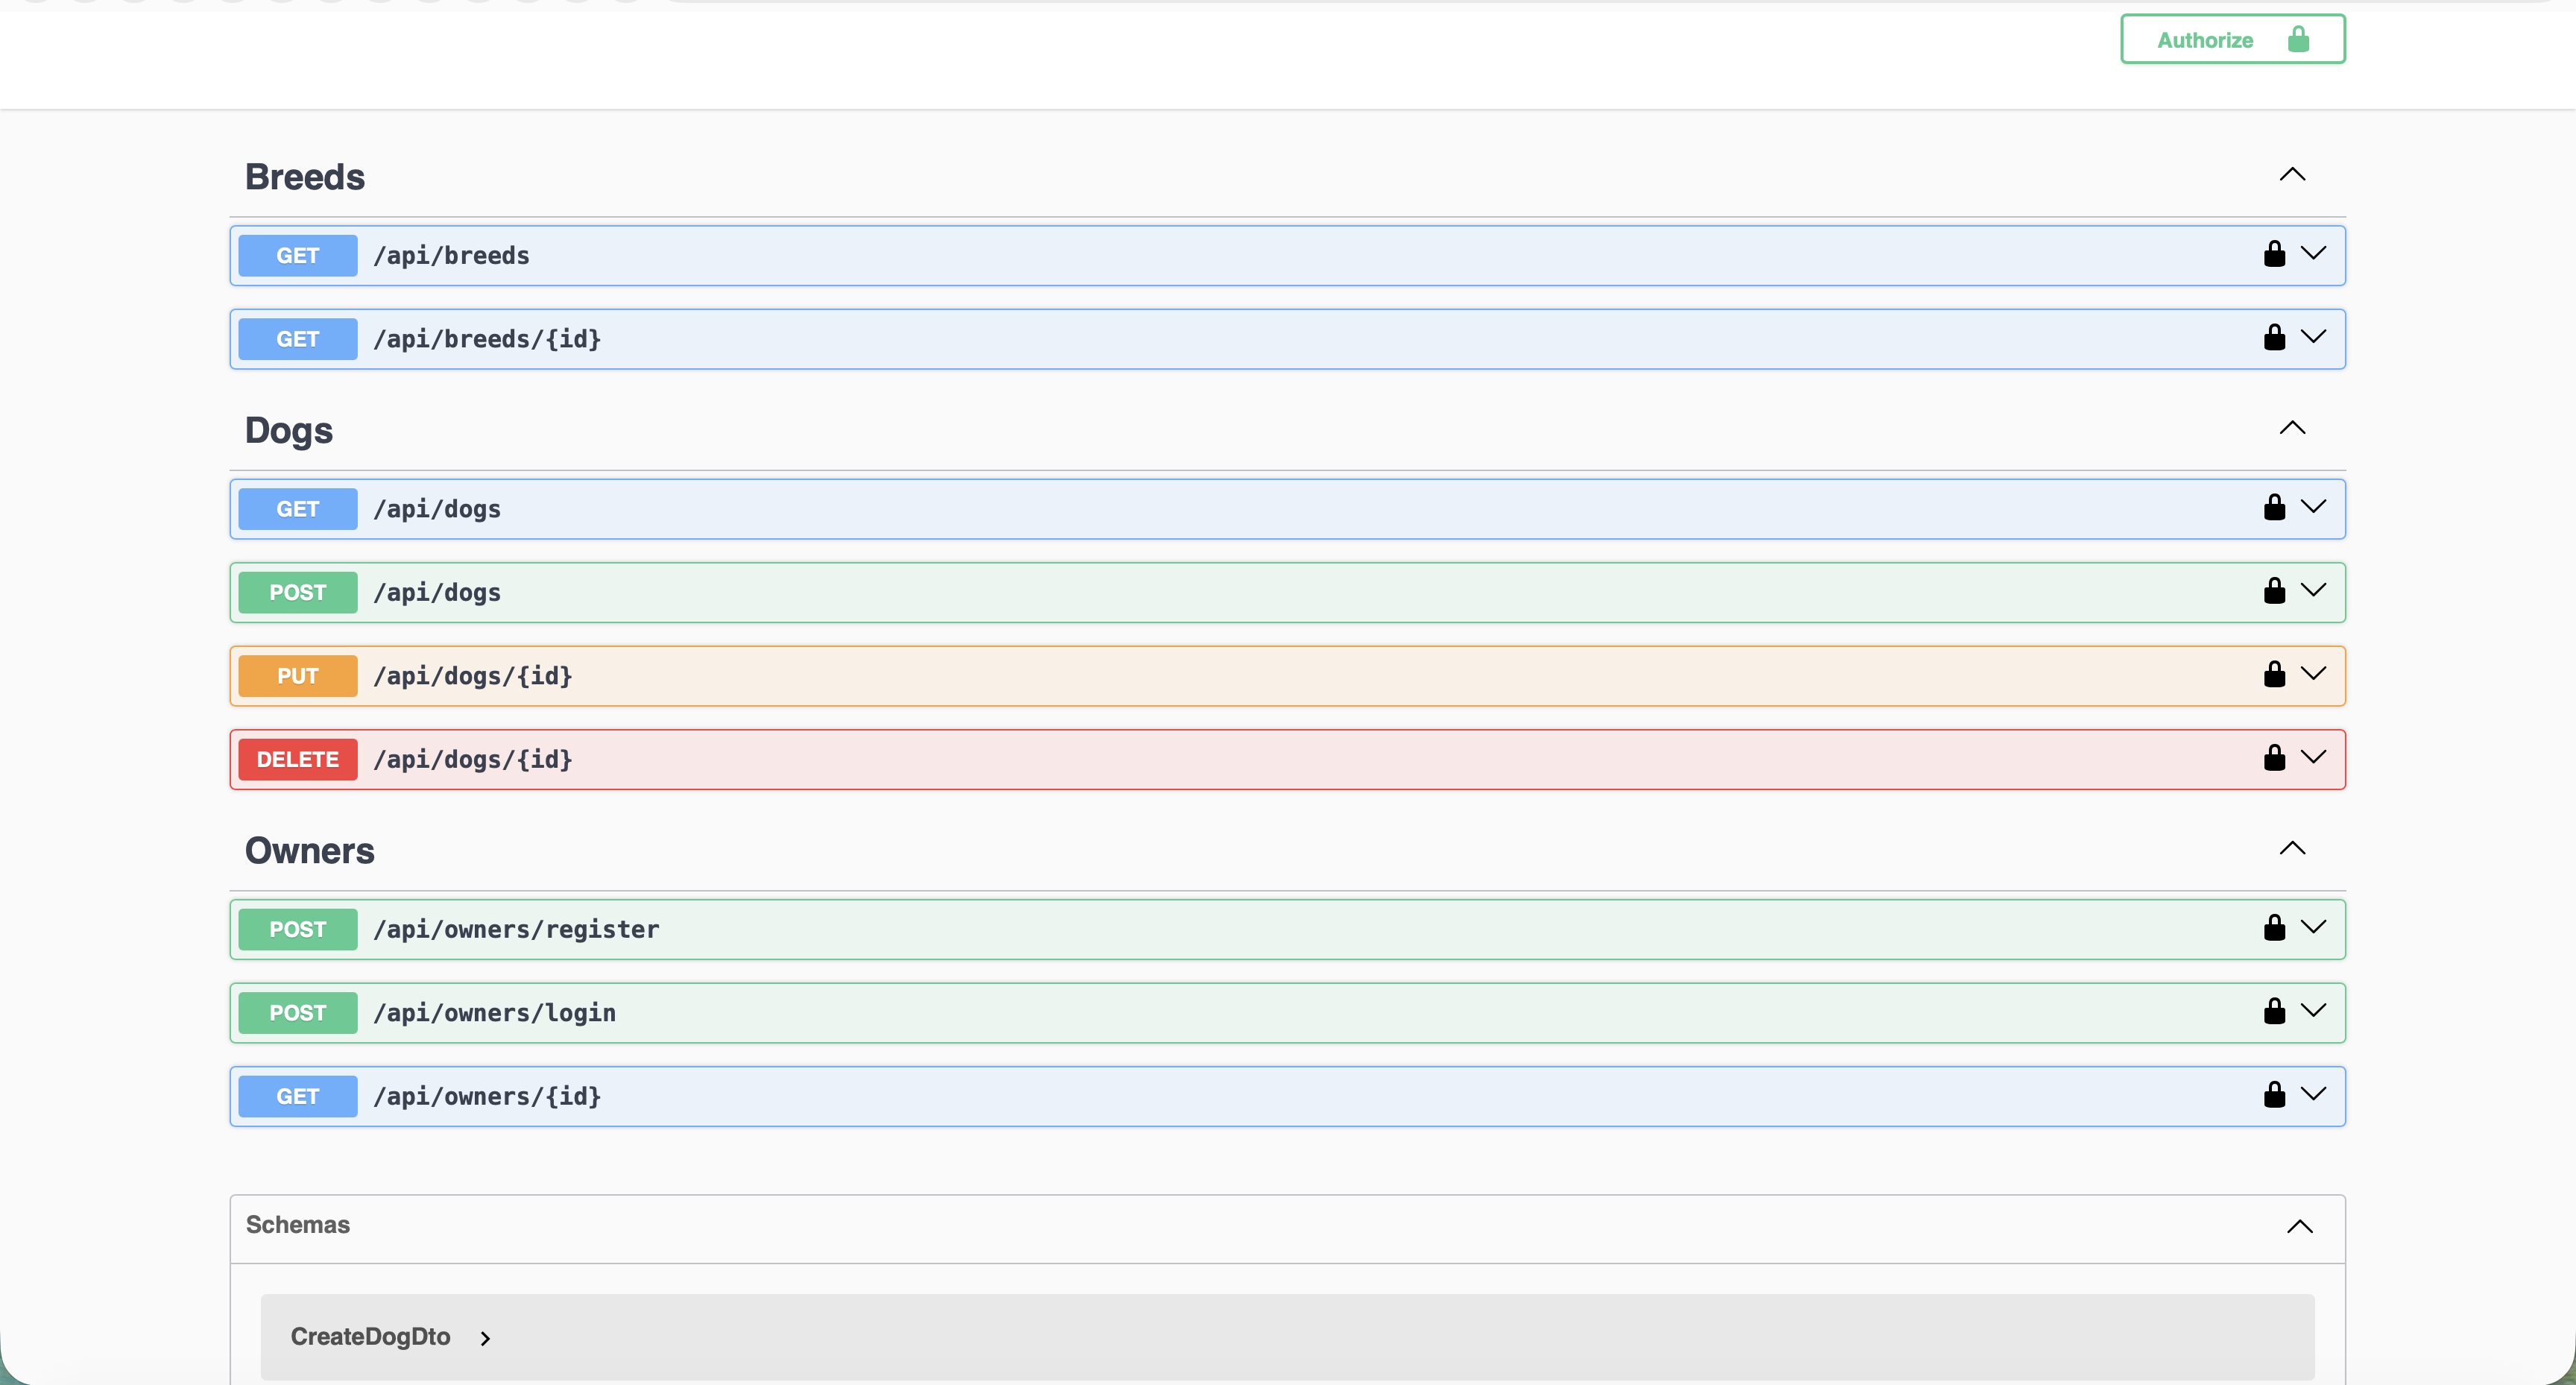
\includegraphics[width=0.9\textwidth]{images/swagger_screenshot.png}
  \caption{Swagger-UI des DoggoGO-Backends}
  \label{fig:swagger}
\end{figure}

%% -------------------------------------------------------
%% Kapitel 6: iOS-Applikation
%% -------------------------------------------------------
\chapter{iOS-Applikation}
\label{chap:ios}

\section{Architektur der iOS-App}
\label{sec:ios-architektur}

Die iOS-Applikation wurde mit \textbf{Swift} und \textbf{SwiftUI} entwickelt und folgt
dem \textbf{MVVM-Muster} (Model-View-ViewModel). Diese Architektur trennt die
UI-Darstellung (View) von der Geschäftslogik und dem Zustand (ViewModel) und erleichtert
Testbarkeit und Wartbarkeit.

\begin{description}
  \item[Model] Entspricht den Datenstrukturen, die der Backend-API entsprechen
    (\texttt{Dog}, \texttt{Owner}, \texttt{Breed}, \texttt{LegalRestrictions}).
  \item[ViewModel] Verwaltet den Zustand der UI mit \texttt{@Published}-Eigenschaften
    und kommuniziert mit dem Backend über HTTP. Durch das \texttt{@StateObject}-Macro
    wird der Lebenszyklus an die View gebunden.
  \item[View] Deklarative SwiftUI-Views lesen den Zustand aus dem ViewModel und reagieren
    automatisch auf Änderungen.
\end{description}

\begin{figure}[H]
  \centering
  \begin{tikzpicture}[
      box/.style={draw, rectangle, rounded corners=4pt,
                  minimum width=4.0cm, minimum height=0.9cm,
                  align=center, font=\small, fill=gray!10, text width=3.8cm},
      ext/.style={draw, rectangle, rounded corners=4pt,
                  minimum width=4.0cm, minimum height=0.9cm,
                  align=center, font=\small, fill=white, dashed, text width=3.8cm},
      arr/.style={{Stealth[length=5pt]}-{Stealth[length=5pt]}, thick},
      oarr/.style={-{Stealth[length=5pt]}, thick, dashed}
    ]
    \node[box] (view)  at (0, 0)   {View\\(SwiftUI)};
    \node[box] (vm)    at (6, 0)   {ViewModel\\(@ObservableObject)};
    \node[box] (model) at (12, 0)  {Model\\(Codable DTOs)};
    \node[ext] (api)   at (6,-2)   {Backend REST-API\\(URLSession)};

    \draw[arr]  (view)  -- node[font=\footnotesize, above]{Bindings} (vm);
    \draw[arr]  (vm)    -- node[font=\footnotesize, above]{Daten}    (model);
    \draw[oarr] (vm)    -- node[font=\footnotesize, right]{HTTP}     (api);
  \end{tikzpicture}
  \caption{MVVM-Architektur der DoggoGO iOS-App}
  \label{fig:mvvm}
\end{figure}

\section{Projektstruktur}
\label{sec:ios-struktur}

Das Xcode-Projekt ist in folgende Gruppen gegliedert:

\begin{itemize}
  \item \texttt{Models/} – \texttt{Codable}-Strukturen für API-DTOs
  \item \texttt{ViewModels/} – \texttt{ObservableObject}-Klassen mit Geschäftslogik
  \item \texttt{Views/} – SwiftUI-Views (Login, Map, DogList, BreedPicker, etc.)
  \item \texttt{Services/} – \texttt{APIService} (HTTP-Kommunikation), \texttt{AuthService}
    (Keychain-Zugriff)
  \item \texttt{Assets.xcassets} – App-Icons, Farbschemata
\end{itemize}

\section{MapKit-Integration}
\label{sec:mapkit}

Die Kartenansicht basiert auf \textbf{MapKit}, Apples nativer Kartenbibliothek. In
SwiftUI wird eine Karte mit \texttt{Map(coordinateRegion:)} eingebunden. Der aktuelle
Standort der Nutzerin / des Nutzers wird über \texttt{CLLocationManager} ermittelt und
als Region übergeben.

\begin{lstlisting}[language=swift, caption={Kartenansicht in SwiftUI (vereinfacht)}, label=lst:mapview, float=h]
import SwiftUI
import MapKit

struct MapView: View {
    @StateObject private var locationManager = LocationManager()
    @State private var region = MKCoordinateRegion(
        center: CLLocationCoordinate2D(
            latitude: 48.2692, longitude: 14.2956), // Leonding
        span: MKCoordinateSpan(
            latitudeDelta: 0.05, longitudeDelta: 0.05)
    )

    var body: some View {
        Map(coordinateRegion: $region,
            showsUserLocation: true,
            annotationItems: locationManager.pois) { poi in
            MapMarker(coordinate: poi.coordinate,
                      tint: poi.color)
        }
        .ignoresSafeArea()
        .onReceive(locationManager.$userLocation) { loc in
            guard let loc else { return }
            region.center = loc.coordinate
        }
    }
}
\end{lstlisting}

Für die Darstellung von Points of Interest (Freilaufwiesen, Sackerlspender,
Hundekot-Mülleimer) werden \texttt{MapMarker}-Annotationen mit farblicher Codierung
pro Kategorie genutzt.

\section{Standortdienste und Berechtigungen}
\label{sec:standortdienste}

Die Standortermittlung wird über \texttt{CLLocationManager} realisiert. Gemäß
DSGVO-Anforderung (NF-03) darf der Standort nur mit expliziter Nutzer\-innen-/Nut\-zer\-zu\-stim\-mung
erfasst werden. Die App fragt beim ersten Start die Berechtigung
\texttt{re\-quest\-When\-In\-Use\-Au\-thor\-iza\-tion()} ab. Die \texttt{Info.plist} enthält die
Pflichteinträge \texttt{NS\-Lo\-ca\-tion\-When\-In\-Use\-Usage\-De\-scrip\-tion} mit einer verständlichen
Begründung.

\begin{lstlisting}[language=swift, caption={LocationManager (Auszug)}, label=lst:locationmanager, float=h]
class LocationManager: NSObject, ObservableObject, CLLocationManagerDelegate {
    private let manager = CLLocationManager()
    @Published var userLocation: CLLocation?

    override init() {
        super.init()
        manager.delegate = self
        manager.desiredAccuracy = kCLLocationAccuracyBest
        manager.requestWhenInUseAuthorization()
        manager.startUpdatingLocation()
    }

    func locationManager(_ manager: CLLocationManager,
                         didUpdateLocations locations: [CLLocation]) {
        userLocation = locations.last
    }
}
\end{lstlisting}

\section{Authentifizierung in der iOS-App}
\label{sec:ios-auth}

\subsection{Login und Registrierung}
\label{subsec:ios-login}

Die Anmeldeansicht (\texttt{LoginView}) enthält Eingabefelder für E-Mail und Passwort.
Nach dem Tippen auf „Anmelden" wird \texttt{POST /api/owners/login} mit den Credentials
aufgerufen. Bei Erfolg liefert das Backend ein JWT zurück:

\begin{lstlisting}[language=swift, caption={Login-Anfrage (Auszug)}, label=lst:login, float=h]
func login(email: String, password: String) async throws {
    let body = LoginRequest(email: email, password: password)
    let response: AuthResponse = try await apiService.post(
        endpoint: "/api/owners/login", body: body)
    AuthService.shared.saveToken(response.token)
    isAuthenticated = true
}
\end{lstlisting}

\subsection{Token-Persistenz im Keychain}
\label{subsec:keychain}

Das JWT wird sicher im iOS~\texttt{Keychain} gespeichert, nicht in
\texttt{UserDefaults}, da der Keychain verschlüsselt und vor anderen Apps geschützt ist.
Der \texttt{AuthService} kapselt alle Keychain-Operationen:

\begin{lstlisting}[language=swift, caption={AuthService – Keychain-Speicherung (Auszug)}, label=lst:keychain, float=h]
class AuthService {
    static let shared = AuthService()
    private let tokenKey = "doggo_jwt_token"

    func saveToken(_ token: String) {
        let data = Data(token.utf8)
        let query: [String: Any] = [
            kSecClass as String: kSecClassGenericPassword,
            kSecAttrAccount as String: tokenKey,
            kSecValueData as String: data
        ]
        SecItemDelete(query as CFDictionary)
        SecItemAdd(query as CFDictionary, nil)
    }

    func getToken() -> String? {
        let query: [String: Any] = [
            kSecClass as String: kSecClassGenericPassword,
            kSecAttrAccount as String: tokenKey,
            kSecReturnData as String: true
        ]
        var item: CFTypeRef?
        guard SecItemCopyMatching(query as CFDictionary, &item) == noErr,
              let data = item as? Data else { return nil }
        return String(data: data, encoding: .utf8)
    }
}
\end{lstlisting}

Beim App-Start prüft das Root-ViewModel, ob ein Token im Keychain vorhanden ist, und
überspringt in diesem Fall die Anmeldeseite direkt zur Kartenansicht.

\section{Hundeprofilverwaltung}
\label{sec:hundeprofil}

Die \texttt{DogListView} listet alle Hunde der angemeldeten Nutzerin / des angemeldeten
Nutzers auf und ruft dazu \texttt{GET /api/dogs} mit dem Bearer-Token auf. Über einen
\texttt{NavigationLink} gelangt man zur Detailansicht oder zum Formular zum Anlegen /
Bearbeiten eines Profils. Die Rassenauswahl erfolgt über einen \texttt{Picker}, der die
von \texttt{GET /api/breeds} geladene Liste anzeigt.

\begin{lstlisting}[language=swift, caption={DogListView – Übersicht der Hundeprofile (Auszug)}, label=lst:doglist, float=h]
struct DogListView: View {
    @StateObject private var viewModel = DogListViewModel()

    var body: some View {
        NavigationView {
            List(viewModel.dogs) { dog in
                NavigationLink(destination: DogDetailView(dog: dog)) {
                    VStack(alignment: .leading) {
                        Text(dog.name).font(.headline)
                        Text("\(dog.breed.breedName), \(dog.age) Jahre")
                            .font(.subheadline).foregroundColor(.secondary)
                    }
                }
            }
            .navigationTitle("Meine Hunde")
            .toolbar {
                ToolbarItem(placement: .navigationBarTrailing) {
                    NavigationLink("Hinzufuegen",
                        destination: AddDogView())
                }
            }
            .task { await viewModel.loadDogs() }
        }
    }
}
\end{lstlisting}

\section{Anzeige gesetzlicher Vorschriften}
\label{sec:ios-legal}

Nach der Rassenauswahl ruft die App \texttt{GET /api/breeds/\{id\}} ab und zeigt die
\texttt{LegalRestrictions} in einer strukturierten Ansicht an. Rassen der Kategorie
\texttt{spezi\-elle\_hun\-de\-rasse} werden farblich hervorgehoben (rotes Label), um die
Nutzerin / den Nutzer auf besondere Pflichten aufmerksam zu machen:

\begin{lstlisting}[language=swift, caption={LegalRestrictionsView – Anzeige der Vorschriften}, label=lst:legal, float=h]
struct LegalRestrictionsView: View {
    let restrictions: LegalRestrictions

    var body: some View {
        VStack(alignment: .leading, spacing: 8) {
            Text("Rechtliche Vorgaben")
                .font(.title2).bold()
            if restrictions.category == "spezielle_hunderasse" {
                Text("Spezielle Hunderasse!")
                    .foregroundColor(.red).bold()
            }
            ForEach(restrictions.rules, id: \.self) { rule in
                Label(rule, systemImage: "exclamationmark.circle")
                    .font(.callout)
            }
        }
        .padding()
    }
}
\end{lstlisting}

\section{HTTP-Kommunikation mit dem Backend}
\label{sec:ios-http}

Alle Netzwerkanfragen werden über einen zentralen \texttt{APIService} abgewickelt, der
\texttt{URLSession} kapselt. Das Bearer-Token wird in jedem Request automatisch als
\texttt{Authorization}-Header eingefügt:

\begin{lstlisting}[language=swift, caption={APIService – Authentifizierter Request (Auszug)}, label=lst:apiservice, float=h]
func get<T: Decodable>(endpoint: String) async throws -> T {
    guard let url = URL(string: baseURL + endpoint) else {
        throw APIError.invalidURL
    }
    var request = URLRequest(url: url)
    if let token = AuthService.shared.getToken() {
        request.setValue("Bearer \(token)",
                         forHTTPHeaderField: "Authorization")
    }
    let (data, response) = try await URLSession.shared.data(for: request)
    guard let http = response as? HTTPURLResponse,
          (200..<300).contains(http.statusCode) else {
        throw APIError.serverError
    }
    return try JSONDecoder().decode(T.self, from: data)
}
\end{lstlisting}

\section{Fehlerbehandlung und Ladezustände}
\label{sec:ios-fehler}

Eine robuste iOS-App muss mit Netzwerkfehlern, ungültigen Tokens und unerwarteten
Serverantworten umgehen. In der DoggoGO-App wird Fehlerbehandlung konsequent im
ViewModel-Layer zentralisiert – die View selbst kennt keine Netzwerklogik.

\subsection{Fehlerdefinition}
\label{subsec:api-error}

Alle möglichen Fehlerszenarien werden in einem \texttt{APIError}-Enum typisiert:

\begin{lstlisting}[language=swift, caption={APIError – Typisierte Fehlerdefinition}, label=lst:apierror]
enum APIError: LocalizedError {
    case invalidURL
    case unauthorized       // 401 – JWT abgelaufen oder ungueltig
    case notFound           // 404 – Ressource nicht vorhanden
    case serverError        // 5xx – Backend-Fehler
    case decodingError      // JSON-Parsing fehlgeschlagen
    case noConnection       // Netzwerk nicht erreichbar

    var errorDescription: String? {
        switch self {
        case .invalidURL:    return "Ungueltige URL."
        case .unauthorized:  return "Sitzung abgelaufen. Bitte erneut anmelden."
        case .notFound:      return "Ressource nicht gefunden."
        case .serverError:   return "Serverfehler. Bitte spaeter versuchen."
        case .decodingError: return "Antwort konnte nicht verarbeitet werden."
        case .noConnection:  return "Keine Internetverbindung."
        }
    }
}
\end{lstlisting}

Das Protokoll \texttt{LocalizedError} stellt sicher, dass SwiftUI und das Betriebssystem
die Fehlerbeschreibung automatisch für Alert-Dialoge verwenden können.

\subsection{Ladezustand und Fehleranzeige im ViewModel}
\label{subsec:loading-state}

Jedes ViewModel hält zwei Zustandsvariablen: \texttt{isLoading} blendet während einer
laufenden Netzwerkanfrage eine Ladeindikator-Ansicht ein, \texttt{errorMessage} speichert
eine lesbare Fehlerbeschreibung für den Alert-Dialog:

\begin{lstlisting}[language=swift, caption={ViewModel – Ladezustand und Fehlerbehandlung}, label=lst:loading]
class DogListViewModel: ObservableObject {
    @Published var dogs: [Dog] = []
    @Published var isLoading = false
    @Published var errorMessage: String?

    func loadDogs() async {
        isLoading = true
        defer { isLoading = false }
        do {
            dogs = try await APIService.shared.get(endpoint: "/api/dogs")
        } catch APIError.unauthorized {
            errorMessage = APIError.unauthorized.errorDescription
            AuthService.shared.deleteToken()   // abgelaufenes Token loeschen
        } catch {
            errorMessage = error.localizedDescription
        }
    }
}
\end{lstlisting}

Das \texttt{defer}-Statement stellt sicher, dass \texttt{isLoading} immer auf
\texttt{false} zurückgesetzt wird – auch wenn die Anfrage mit einem Fehler endet.
Bei einem \texttt{401~Unauthorized} wird das gespeicherte JWT automatisch gelöscht,
sodass die Nutzerin / der Nutzer zur Anmeldeseite weitergeleitet wird.

\subsection{Alert-Anzeige in der View}
\label{subsec:alert}

Die View abonniert \texttt{errorMessage} über ein \texttt{.alert}-Modifier und zeigt
bei gesetztem Wert automatisch einen Dialog an:

\begin{lstlisting}[language=swift, caption={SwiftUI – Alert fuer Fehlermeldungen}, label=lst:alert]
.alert("Fehler", isPresented: Binding(
    get: { viewModel.errorMessage != nil },
    set: { if !$0 { viewModel.errorMessage = nil } }
)) {
    Button("OK", role: .cancel) { }
} message: {
    Text(viewModel.errorMessage ?? "")
}
.overlay {
    if viewModel.isLoading {
        ProgressView("Laden ...")
            .padding()
            .background(.regularMaterial, in: RoundedRectangle(cornerRadius: 8))
    }
}
\end{lstlisting}

Dieser Ansatz hält die View vollständig frei von Fehlerlogik: Sie bindet lediglich den
Zustand des ViewModels und delegiert jede Entscheidung dorthin.

%% -------------------------------------------------------
%% Kapitel 7: Testing und Deployment
%% -------------------------------------------------------
\chapter{Testing und Deployment}
\label{chap:testing}

\section{Teststrategie}
\label{sec:teststrategie}

Eine systematische Teststrategie stellt sicher, dass das Backend und die iOS-App korrekt
funktionieren und die definierten Anforderungen erfüllen. Für DoggoGO wurden drei
Testebenen eingesetzt:

\begin{enumerate}
  \item \textbf{Manuelle API-Tests} über Swagger~UI und Postman
  \item \textbf{Unit-Tests} für einzelne Backend-Komponenten (xUnit)
  \item \textbf{Integrationstests} für das Zusammenspiel zwischen iOS-App und Backend
\end{enumerate}

\section{Backend-Tests}
\label{sec:backend-tests}

\subsection{Manuelle Tests mit Swagger und Postman}
\label{subsec:swagger-tests}

Während der Entwicklung wurden alle API-Endpunkte zunächst manuell über die
\textbf{Swagger-UI} getestet. Dies erlaubt schnelles Feedback ohne Testrahmenaufwand:
Registrierung, Anmeldung, CRUD-Operationen für Hunde sowie das Abrufen der Rassenliste
wurden iterativ überprüft. Für komplexere Szenarien (z.\,B.\ Fehlerfälle, ungültige Tokens)
wurde \textbf{Postman} mit einer gespeicherten Collection genutzt, die die wichtigsten
Endpunkte mit vorbereiteten Request-Bodies enthält.

Tabelle~\ref{tab:test-szenarien} listet die wichtigsten getesteten Szenarien auf:

\begin{table}[H]
  \centering
  \caption{Getestete API-Szenarien}
  \label{tab:test-szenarien}
  \small
  \begin{tabularx}{\textwidth}{|l|l|Y|l|}
    \hline
    \textbf{Szenario} & \textbf{Endpunkt} & \textbf{Erwartetes Ergebnis} &
    \textbf{Status} \\
    \hline
    Registrierung (gültig)     & POST /owners/register & 201 Created, Owner-Objekt    & OK \\
    \hline
    Registrierung (doppelt)    & POST /owners/register & 409 Conflict (doppelte Email) & OK \\
    \hline
    Anmeldung (gültig)         & POST /owners/login    & 200 OK, JWT                  & OK \\
    \hline
    Anmeldung (Falsches PW)    & POST /owners/login    & 401 Unauthorized             & OK \\
    \hline
    Hund anlegen (auth.)       & POST /api/dogs        & 201 Created, Dog-Objekt      & OK \\
    \hline
    Hund anlegen (unauth.)     & POST /api/dogs        & 401 Unauthorized             & OK \\
    \hline
    Hund löschen (Cascade)     & DELETE /owners/\{id\} & 204 + Hunde gelöscht         & OK \\
    \hline
    Rassen abrufen             & GET /api/breeds       & 200 OK, Rassenliste mit Regeln & OK \\
    \hline
  \end{tabularx}
\end{table}

\subsection{Unit-Tests mit xUnit}
\label{subsec:xunit}

Für die Passwort-Hashing-Logik und die JWT-Erzeugung wurden Unit-Tests mit
\textbf{xUnit} implementiert. Listing~\ref{lst:unittest} zeigt einen exemplarischen Test
für den Passwort-Hash-Vergleich:

\begin{lstlisting}[language=csharp, caption={xUnit-Test – Passwort-Hash-Verifikation}, label=lst:unittest, float=htbp]
public class PasswordHashTests
{
    [Fact]
    public void VerifyPassword_CorrectPassword_ReturnsTrue()
    {
        // Arrange
        using var hmac = new HMACSHA512();
        var salt = hmac.Key;
        var hash = hmac.ComputeHash(Encoding.UTF8.GetBytes("Test1234!"));

        // Act
        using var hmac2 = new HMACSHA512(salt);
        var verifyHash = hmac2.ComputeHash(
            Encoding.UTF8.GetBytes("Test1234!"));

        // Assert
        Assert.Equal(hash, verifyHash);
    }

    [Fact]
    public void VerifyPassword_WrongPassword_ReturnsFalse()
    {
        using var hmac = new HMACSHA512();
        var salt = hmac.Key;
        var hash = hmac.ComputeHash(Encoding.UTF8.GetBytes("Test1234!"));

        using var hmac2 = new HMACSHA512(salt);
        var verifyHash = hmac2.ComputeHash(
            Encoding.UTF8.GetBytes("WrongPassword"));

        Assert.NotEqual(hash, verifyHash);
    }
}
\end{lstlisting}

\section{iOS-Tests}
\label{sec:ios-tests}

Die iOS-App wurde mit \textbf{XCTest} getestet. Aufgrund des Umfangs der Diplomarbeit
konzentrierten sich die Tests auf das \texttt{AuthService}-Modul (Keychain-Operationen)
und die \texttt{APIService}-Klasse (URL-Konstruktion, Fehlerbehandlung):

\begin{lstlisting}[language=swift, caption={XCTest – AuthService Keychain-Test}, label=lst:xctest, float=htbp]
class AuthServiceTests: XCTestCase {

    func testSaveAndRetrieveToken() {
        let service = AuthService.shared
        let testToken = "eyJhbGciOiJIUzI1NiIsInR5cCI6IkpXVCJ9.test"

        service.saveToken(testToken)
        let retrieved = service.getToken()

        XCTAssertEqual(testToken, retrieved)
    }

    func testDeleteToken() {
        let service = AuthService.shared
        service.saveToken("some.token.value")
        service.deleteToken()

        XCTAssertNil(service.getToken())
    }
}
\end{lstlisting}

\section{Integrationstests}
\label{sec:integrationstests}

Integrationstests überprüften das Ende-zu-Ende-Verhalten des Gesamtsystems: Die iOS-App
wird im Simulator gestartet, und die Benutzerabläufe (Registrierung → Anmeldung →
Hundeprofi anlegen → Rasse mit Rechtsvorschriften abrufen) werden manuell durchgeführt.
Die HTTP-Anfragen wurden dabei mit dem Netzwerk-Inspector in Xcode beobachtet, um
korrekte Request/Response-Zyklen zu verifizieren.

\section{Deployment-Verifikation}
\label{sec:deployment-test}

Nach einem \texttt{docker compose up --build} wurden folgende Punkte geprüft:

\begin{itemize}
  \item PostgreSQL-Container läuft und ist über Port~5432 erreichbar.
  \item Backend-Container startet, Datenbankmigrationen werden ohne Fehler angewendet.
  \item Breed-Seeding protokolliert \textit{„Breeds seeded successfully"}.
  \item Swagger-UI ist unter \texttt{http://localhost:8080/swagger} erreichbar.
  \item Registrierung und Anmeldung über Swagger-UI funktionieren korrekt.
\end{itemize}

%% -------------------------------------------------------
%% Kapitel 8: Zusammenfassung
%% -------------------------------------------------------
\chapter{Zusammenfassung}
\label{chap:zusammenfassung}

\section{Erreichte Ziele}
\label{sec:erreichte-ziele}

Im Rahmen dieser Diplomarbeit wurden die beiden zentralen Komponenten von DoggoGO –
Backend und iOS-Applikation – konzipiert und implementiert.

Das \textbf{Backend} auf Basis von ASP.NET~Core~8 stellt eine vollständige RESTful~API
mit Registrierung, JWT-Authentifizierung, Hundeprofilverwaltung und Rassendatenverwaltung
bereit. Die Datenhaltung erfolgt über PostgreSQL mit EF~Core~9; das automatische
Breed-Seeding aus einer JSON-Datei macht die Rassen-Datenbank sofort nutzbar. Das
gesamte System ist mittels Docker~Compose containerisiert und damit plattformunabhängig
deploybar.

Die \textbf{iOS-App} bietet eine kartenbasierte Darstellung des Benutzerstandorts
(MapKit), sichere JWT-Authentifizierung mit Keychain-Persistenz, Hundeprofilverwaltung
sowie die Anzeige rassenspezifischer Rechtsvorschriften. Die MVVM-Architektur mit
SwiftUI ermöglicht eine klare Trennung von Darstellung und Logik.

Alle in Kapitel~\ref{chap:anforderungen} definierten funktionalen Anforderungen
(FA-B01 bis FA-B08 und FA-I01 bis FA-I08) wurden erfüllt. Die nicht-funktionalen
Anforderungen bezüglich Sicherheit (NF-01, NF-02), Datenschutz (NF-03) und
Portierbarkeit (NF-06) wurden ebenfalls umgesetzt.

\section{Suboptimale Entscheidungen}
\label{sec:suboptimal}

Im Rückblick lassen sich einige Entscheidungen identifizieren, die bei einer Neuentwicklung
anders getroffen würden:

\paragraph{Doppelter Foreign-Key in der Initialmigration}
Die automatisch generierte EF~Core-Migration \texttt{InitDatabase} enthielt einen
redundanten Foreign-Key \texttt{Legal\-Restrictions\-Id1} in der \texttt{Breeds}-Tabelle.
Dieser entstand durch eine nicht klar definierte \texttt{WithMany()}-Konfiguration und
musste manuell aus der Migration entfernt werden. Eine sorgfältigere Konfiguration in
\texttt{OnModelCreating} hätte diesen Fehler vermieden.

\paragraph{Fehlendes Con\-trol\-ler-Layer}
Das Backend wurde zunächst ohne dedizierte Con\-trol\-ler-Klas\-sen begonnen; Endpunkte wurden
direkt in \texttt{Program.cs} als Minimal~API definiert. Erst im Verlauf des Projekts
wurde auf den klassischen Con\-trol\-ler-An\-satz umgestellt, was zu einer Umstrukturierung
des Codes führte. Ein frühzeitiger Entschluss für einen der beiden Ansätze hätte Zeit
gespart.

\paragraph{Fehlende Input-Validierung}
In der aktuellen Version werden Eingaben (z.\,B.\ beim Anlegen eines Hundes) nicht
serverseitig mit \texttt{DataAnnotations} oder einem Validierungsframework validiert.
Ungültige Werte (leerer Name, negatives Alter) könnten so in die Datenbank gelangen.
Für eine produktive Anwendung ist eine umfassende Validierungsschicht zwingend erforderlich.

\paragraph{iOS-Simulator statt echtes Gerät}
Die iOS-App wurde ausschließlich im Xcode-Simulator getestet. GPS-Standortdaten wurden
simuliert. Tests auf einem physischen Gerät hätten möglicherweise Probleme mit der
Standortgenauigkeit oder Keychain-Berechtigungen aufgedeckt.

\section{Einschränkungen der Lösung}
\label{sec:einschraenkungen}

\begin{itemize}
  \item \textbf{Keine echten Geo-Daten:} Freilaufwiesen, Sackerlspender und
    Hundekot-Mülleimer sind im aktuellen Stand nicht in der Datenbank enthalten.
    Die Kartendarstellung zeigt ausschließlich den Benutzerstandort. Die Entitäten und
    API-Endpunkte für Standortdaten wurden geplant, konnten im Rahmen der Diplomarbeit
    aber nicht vollständig implementiert werden.
  \item \textbf{Nur iOS, kein Android:} Eine Android-App ist nicht Teil des Projekts.
    Die API-Architektur ist jedoch so gestaltet, dass ein Android-Client ohne
    Backend-Änderungen ergänzt werden könnte.
  \item \textbf{Keine Produktionsumgebung:} Das System wurde für Entwicklungs- und
    Demonstrationszwecke konfiguriert. Für einen produktiven Betrieb wären HTTPS-Terminierung,
    Secrets-Management (z.\,B.\ Vault) und ein Reverse-Proxy (Nginx) notwendig.
  \item \textbf{Regionale Begrenzung:} Die Rechtsvorschriften sind derzeit auf
    österreichisches Recht (Wiener Hundegesetz) beschränkt. Eine Ausweitung auf andere
    Bundesländer oder Länder erfordert weitere Datenerhebung und -pflege.
\end{itemize}

\section{Erweiterungsmöglichkeiten}
\label{sec:erweiterungen}

Das System bietet eine solide Basis für zahlreiche Erweiterungen:

\begin{description}
  \item[Standort-Daten (DOG3–DOG5, DOG17)]
    Import von Open-Data-Geodaten (z.\,B.\ der Stadt Wien) für Freilaufwiesen,
    Sackerlspender und Hundewaschstationen. Neue \texttt{Location}-Entität im Backend,
    REST-Endpunkte für Geo-Abfragen.
  \item[Geofencing-Benachrichtigungen (DOG11)]
    Push-Benachrichtigungen via APNs, wenn die Nutzerin / der Nutzer eine Zone mit
    besonderen Vorschriften betritt. Serverseitig über einen Background-Worker realisierbar.
  \item[Routenplanung (DOG14)]
    Integration von MapKit-Routing zur Navigation zur nächsten Freilaufwiese.
  \item[Favoriten (DOG15)]
    Persistenz von Lieblings-Standorten in der Datenbank.
  \item[Android-App]
    Da die REST-API plattformunabhängig ist, kann ein Android-Client (Kotlin / Jetpack
    Compose) ohne Backend-Änderungen ergänzt werden.
  \item[Community-Features]
    Nutzerbewertungen und Erfahrungsberichte zu Standorten (neue Entitäten \texttt{Review},
    \texttt{Report}).
\end{description}


%% -------------------------------------------------------
%% Literaturverzeichnis
%% -------------------------------------------------------
\printbibliography[heading=bibintoc, title={Literaturverzeichnis}]

%% -------------------------------------------------------
%% Anhang
%% -------------------------------------------------------
\appendix
%% -------------------------------------------------------
%% Anhang A: API-Spezifikation
%% -------------------------------------------------------
\chapter{API-Endpunkte im Detail}
\label{app:api}

Dieser Anhang listet alle implementierten und geplanten REST-Endpunkte der
DoggoGO-Backend-API mit Request/Response-Schemata auf. Die vollständige und interaktive
Dokumentation ist über die Swagger-UI unter \texttt{/swagger} erreichbar.

\section*{Authentifizierung}

\textbf{POST /api/owners/register}

\begin{itemize}
  \item \textbf{Beschreibung:} Registriert eine neue Nutzerin / einen neuen Nutzer.
  \item \textbf{Request-Body (JSON):}
\end{itemize}
\begin{lstlisting}[language={}]
{
  "name": "Max Muster",
  "email": "max@example.com",
  "password": "SecurePass123!",
  "phoneNumber": "+43 123 456789"
}
\end{lstlisting}
\begin{itemize}
  \item \textbf{Response 201:} Owner-Objekt (ohne Passwort-Felder)
  \item \textbf{Response 409:} E-Mail bereits vergeben
\end{itemize}

\vspace{1em}
\textbf{POST /api/owners/login}
\begin{itemize}
  \item \textbf{Beschreibung:} Meldet eine Nutzerin / einen Nutzer an und gibt ein JWT zurück.
  \item \textbf{Request-Body (JSON):}
\end{itemize}
\begin{lstlisting}[language={}]
{
  "email": "max@example.com",
  "password": "SecurePass123!"
}
\end{lstlisting}
\begin{itemize}
  \item \textbf{Response 200:} \texttt{\{"token": "eyJ...\}"}
  \item \textbf{Response 401:} Ungültige Anmeldedaten
\end{itemize}

\section*{Hunde (Dogs)}

\textbf{GET /api/dogs} \quad \textit{(Authentifizierung erforderlich)}\\
Gibt alle Hundeprofile der aktuellen Nutzerin / des aktuellen Nutzers zurück.

\textbf{POST /api/dogs} \quad \textit{(Authentifizierung erforderlich)}\\
Legt ein neues Hundeprofil an.
\begin{lstlisting}[language={}]
{
  "name": "Bello",
  "age": 3,
  "breedId": "a1b2c3d4-..."
}
\end{lstlisting}

\textbf{PUT /api/dogs/\{id\}} \quad \textit{(Authentifizierung erforderlich)}\\
Aktualisiert ein bestehendes Hundeprofil.

\textbf{DELETE /api/dogs/\{id\}} \quad \textit{(Authentifizierung erforderlich)}\\
Löscht ein Hundeprofil.

\section*{Hunderassen (Breeds)}

\textbf{GET /api/breeds}\\
Gibt alle Hunderassen inklusive \texttt{LegalRestrictions} zurück.

\textbf{GET /api/breeds/\{id\}}\\
Gibt eine einzelne Rasse mit vollständigen Rechtsvorschriften zurück.

%% -------------------------------------------------------
%% Anhang B: Dokumentation der KI-Nutzung
%% -------------------------------------------------------
\chapter{Dokumentation der KI-Nutzung}
\label{app:ki}

Gemäß den Richtlinien der HTL Leonding müssen alle im Rahmen dieser Diplomarbeit
verwendeten KI-generierten Inhalte dokumentiert werden. Die folgende Tabelle listet
alle Einsätze auf, bei denen ein KI-Tool zur Unterstützung herangezogen wurde.

\begin{longtable}{|p{0.12\textwidth}|p{0.25\textwidth}|p{0.35\textwidth}|p{0.18\textwidth}|}
  \hline
  \textbf{Datum} & \textbf{KI-Tool} & \textbf{Verwendungszweck / Prompt (Zusammenfassung)} &
  \textbf{Kapitel / Datei} \\
  \hline
  \endfirsthead
  \hline
  \textbf{Datum} & \textbf{KI-Tool} & \textbf{Verwendungszweck} & \textbf{Kapitel} \\
  \hline
  \endhead
  % Einträge hier ergänzen – Beispiel:
  [Datum] & Claude (Anthropic) &
  Strukturvorschlag für Kapitel Systemarchitektur; Überarbeitung auf Basis eigener
  Inhalte und Projektcode &
  Kap.~\ref{chap:architektur} \\
  \hline
  [Datum] & Claude (Anthropic) &
  Vorlage für JWT-Authentifizierungslogik; angepasst an eigene Modelle und Konfiguration &
  Kap.~\ref{chap:backend} \\
  \hline
  [Datum] & Claude (Anthropic) &
  Entwurf der SwiftUI-Listings; geprüft und an eigene Projektstruktur angepasst &
  Kap.~\ref{chap:ios} \\
  \hline
  \multicolumn{4}{|p{0.9\textwidth}|}{
    \textit{Alle KI-generierten Inhalte wurden kritisch geprüft, inhaltlich angepasst
    und auf ihre Korrektheit hin verifiziert. Die endgültige Verantwortung für den Inhalt
    liegt beim Autor dieser Arbeit.}
  } \\
  \hline
\end{longtable}


\end{document}
